\documentclass[11pt,letterpaper]{article}
\usepackage{fontspec}
\setmainfont{texgyrepagella}[Extension=.otf,UprightFont=*-regular,BoldFont=*-bold,ItalicFont=*-italic,BoldItalicFont=*-bolditalic]
\usepackage[bidi=default]{babel}
\babelprovide[import,main]{spanish}
\babelprovide[import]{hebrew}
\babelprovide[import]{ancientgreek}
\babelfont[hebrew]{rm}[Path=fonts/,BoldFont=NotoHebrewSerif-700.ttf,Scale=0.95]{NotoHebrewSerif-400.ttf}
\babelfont[ancientgreek]{rm}[Path=fonts/]{GFSPorson.otf}
\newcommand{\heb}[1]{\mbox{\foreignlanguage{hebrew}{#1}}}
\newcommand{\grc}[1]{\foreignlanguage{ancientgreek}{#1}}
\newcommand{\hebverso}[1]{\par\smallskip{\centering\begin{otherlanguage}{hebrew}\large #1\end{otherlanguage}\par}\smallskip}
\newcommand{\SENOR}{\textsc{Señor}}
\usepackage[margin=2.5cm,headheight=14pt]{geometry}
\usepackage{microtype,ragged2e,booktabs,graphicx,xcolor,csquotes,array}
\usepackage[hidelinks]{hyperref}\usepackage{xurl}\urlstyle{same}
\usepackage[most]{tcolorbox}
\usepackage{tikz}\usetikzlibrary{arrows.meta,positioning,calc,decorations.pathreplacing}
\usepackage{titlesec,fancyhdr}
\definecolor{azul}{HTML}{15437C}\definecolor{azuloscuro}{HTML}{0B1F3A}\definecolor{celeste}{HTML}{5694D6}
\definecolor{dorado}{RGB}{196,154,60}\definecolor{papiro}{RGB}{246,239,220}\definecolor{gris}{RGB}{70,78,96}
\titleformat{\section}{\Large\bfseries\color{azul}}{\thesection.}{0.6em}{}
\titleformat{\subsection}{\large\bfseries\color{azuloscuro}}{\thesubsection}{0.6em}{}
\pagestyle{fancy}\fancyhf{}
\fancyhead[L]{\foreignlanguage{spanish}{\small\itshape\color{gris}El Dios que llena el cielo y la tierra}}\fancyhead[R]{\foreignlanguage{spanish}{\small\color{gris}\thepage}}
\renewcommand{\headrulewidth}{0.4pt}
\setlength{\parindent}{1.27cm}\linespread{1.15}\setlength{\emergencystretch}{3em}
\newtcolorbox{cita}[1][]{enhanced,colback=azul!6!white,colframe=azul,boxrule=0pt,leftrule=2.5pt,arc=0pt,
  left=8pt,right=8pt,top=5pt,bottom=5pt,before skip=8pt,after skip=8pt,fontupper=\itshape,#1}
\newcommand{\fuente}[1]{\par\hfill{\upshape\bfseries\small\textcolor{azul}{#1}}}
\newtcolorbox{nota}[1][]{enhanced,colback=dorado!10,colframe=dorado!85!azul,boxrule=0.6pt,arc=2pt,
  fonttitle=\bfseries\small,coltitle=azuloscuro,colbacktitle=dorado!30,fontupper=\small,title={#1}}
\newtcolorbox{filologia}[1][]{enhanced,colback=white,colframe=azul!45,boxrule=0.5pt,arc=2pt,
  fonttitle=\bfseries\small,coltitle=white,colbacktitle=azul!80,fontupper=\small,title={Filología: #1}}
\newcommand{\refapa}[1]{\par{\RaggedRight\hangindent=1.27cm\hangafter=1\noindent #1\par}\vspace{4pt}}
\newcommand{\destacar}[1]{\textbf{\textcolor{azul}{#1}}}
\newcolumntype{L}[1]{>{\RaggedRight\arraybackslash}p{#1}}


\title{\color{azul}\bfseries El Dios que llena el cielo y la tierra\\[4pt]\large\color{gris}\mdseries ``¿No lleno yo, dice \SENOR{}, el cielo y la tierra?'' (Jer 23:24)}
\author{}\date{}
\begin{document}
\maketitle\thispagestyle{empty}

\begin{abstract}\noindent
La pregunta ``¿Dónde está tu Dios?'' (Sal 42:3) atraviesa la Escritura de un extremo al otro. Este capítulo estudia la respuesta que Dios mismo da por medio de Jeremías: ``¿Soy yo Dios de cerca solamente\ldots{} y no Dios desde muy lejos?\ldots{} ¿No lleno yo\ldots{} el cielo y la tierra?'' (Jer 23:23--24). Parte de ese texto, pronunciado contra profetas que creían poder hablar en nombre de Dios sin ser vistos por él, y compara su lectura en el texto masorético, la Septuaginta y el Targum. Puesto que el hebreo carece de una palabra para ``omnipresencia'', el estudio recorre el vocabulario con que Israel nombra la presencia, \emph{panim} (rostro), \emph{sham} (allí), \emph{im} (con), \emph{qarov} (cerca), \emph{maqom} (lugar), \emph{male'} (llenar) y \emph{kul} (contener), y sigue su paso al griego de Pablo. El Nombre que revela el atributo es \SENOR{}-sama, ``el \SENOR{} está allí'' (Ez 48:35), cumplido en Emanuel, ``Dios con nosotros'' (Is 7:14; Mt 1:23). A partir de allí el capítulo define el atributo, distingue inmensidad y omnipresencia junto con los modos de la presencia divina, y lo expone desde la Escritura: Dios está presente porque es Espíritu, porque es inmenso, porque reina en todo lugar y porque su mirada no deja nada fuera, con el apoyo de Agustín, Charnock, Berkhof y Washer. El encuentro en la historia de Israel es Betel, donde Jacob, en plena huida, descubre que ``el \SENOR{} está en este lugar, y yo no lo sabía'' (Gn 28:16). Se recoge luego la mirada del judaísmo (Dios llamado \emph{HaMaqom}, ``el Lugar''; la Shejiná que no deja lugar vacío; la \emph{Qedushá}; los targumes; Maimónides; Qumrán) y se lee el atributo en Cristo con Pablo: el Dios no lejano de Atenas (Hch 17:27--28), Cristo que ``todo lo llena en todo'' (Ef 1:23; 4:10), la palabra cercana (Ro 10:6--8), el templo que es un pueblo (1 Co 3:16) y ``el Señor está cerca'' (Flp 4:5). El capítulo termina con lo que significa vivir delante de Dios.
\par\smallskip\noindent\textbf{Palabras clave:} omnipresencia, inmensidad, presencia, \emph{panim}, \emph{maqom}, \emph{HaMaqom}, Shejiná, Betel, Emanuel, \emph{coram Deo}.\end{abstract}

\begin{nota}[Nota sobre el texto]
Las citas bíblicas son de la Reina-Valera 1960. Donde esta escribe ``Jehová'', aquí se escribe \SENOR, que traduce el tetragrama \heb{יהוה}, leído en la tradición judía como \emph{Adonay}. El hebreo sigue la BHS; el griego, NA28 y la Septuaginta de Rahlfs-Hanhart. Las fuentes judías (Midrash, Talmud, Targum, liturgia, Maimónides) se citan desde Sefaria con traducción propia, y todo lo que es interpretación se marca como precisión. Cuando la numeración hebrea o griega difiere de la española, se indica entre corchetes.
\end{nota}

%===================================================================
\section{¿Dónde está Dios?}

Dos veces en un mismo salmo el creyente oye la burla: ``Fueron mis lágrimas mi pan de día y de noche, mientras me dicen todos los días: ¿Dónde está tu Dios?'' (Sal 42:3; cf. 42:10). Las naciones repiten la pregunta, y el pueblo tiene preparada su respuesta:

\begin{cita}¿Por qué han de decir las gentes: ¿Dónde está ahora su Dios? Nuestro Dios está en los cielos; Todo lo que quiso ha hecho.\fuente{(Sal 115:2--3)}\end{cita}

La respuesta bíblica tiene dos caras, y nunca las separa. Dios está \destacar{en los cielos}, por encima de todo y sin depender de nada; y a la vez está \destacar{aquí}, tan cerca que nadie puede esconderse de él. Moisés reunió ambas en una sola frase: ``Aprende pues, hoy, y reflexiona en tu corazón que \SENOR{} es Dios arriba en el cielo y abajo en la tierra, y no hay otro'' (Dt 4:39). Y la misma confesión salió de labios de Rahab, una cananea de Jericó (Jos 2:11).

La palabra ``omnipresente'' no aparece en la Biblia. Procede del latín \emph{omnipraesens} (\emph{omnis}, ``todo'', y \emph{praesens}, ``presente'') y, como resume Washer (2021), ``cuando la Biblia afirma que Dios es omnipresente, quiere decir que Él siempre está presente en todo lugar en toda Su plenitud'' (p. 89). El término es teológico; la verdad que nombra recorre la Escritura de punta a punta.

\begin{center}
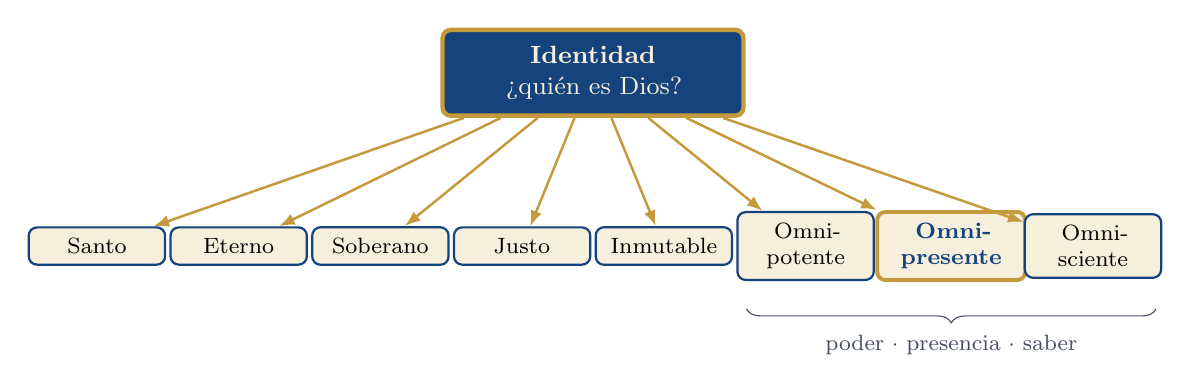
\begin{tikzpicture}[font=\small,
  caja/.style={draw=azul,line width=0.8pt,fill=papiro,rounded corners=3pt,inner sep=4pt,align=center}]
 \node[draw=dorado,line width=1.6pt,fill=azul,text=papiro,rounded corners=3pt,text width=3.4cm,align=center,inner sep=6pt] (s) at (0,2.0) {\textbf{Identidad}\\ ¿quién es Dios?};
 \foreach \x/\n/\t in {-6.3/a/Santo, -4.5/b/Eterno, -2.7/c/Soberano, -0.9/d/Justo, 0.9/e/Inmutable, 2.7/f/{Omni-\\potente}}{
   \node[caja,text width=1.45cm,font=\footnotesize] (\n) at (\x,-0.2) {\t};
   \draw[-{Latex[length=2mm]},dorado,line width=0.9pt](s)--(\n);}
 \node[draw=dorado,line width=1.4pt,fill=papiro,rounded corners=3pt,text width=1.6cm,align=center,inner sep=4pt,font=\footnotesize] (g) at (4.55,-0.2) {\textbf{\textcolor{azul}{Omni-}}\\\textbf{\textcolor{azul}{presente}}};
 \node[caja,text width=1.45cm,font=\footnotesize] (h) at (6.35,-0.2) {Omni-\\sciente};
 \draw[-{Latex[length=2mm]},dorado,line width=0.9pt](s)--(g); \draw[-{Latex[length=2mm]},dorado,line width=0.9pt](s)--(h);
 \draw[decorate,decoration={brace,amplitude=5pt,mirror},gris] (1.95,-1.0)--(7.15,-1.0) node[midway,below=6pt,font=\footnotesize,text=gris]{poder $\cdot$ presencia $\cdot$ saber};
\end{tikzpicture}\par
{\footnotesize\color{gris}\textit{Figura 1.} El atributo dentro de la Parte II (Identidad). \textit{Nota.} Elaboración propia según la clasificación de la serie.}
\end{center}

La omnipresencia forma con la omnipotencia y la omnisciencia una tríada que la tradición ha estudiado junta. Charnock las reúne en una sola frase: ``Como su esencia es inmensa, no puede ser confinada en un lugar; como es eterno, no puede medirse en el tiempo; así que como es todopoderoso, no puede ser limitado en lo que respecta a la acción'' (citado en Pink, 2020, cap. 9, p. 47). El capítulo anterior estudió el poder y el siguiente estudiará el saber; este se ocupa de la presencia: el Dios que puede todo y sabe todo \destacar{está} en todo.

\begin{nota}[Precisión]
Clasificación propuesta: atributo de la Identidad; \emph{incomunicable}. Ninguna criatura está en más de un lugar a la vez; solo Dios llena el cielo y la tierra (Jer 23:24). Lo que sí se comunica es su presencia: Dios habita en su pueblo (1 Co 3:16), y el creyente vive ``delante de Dios''.
\end{nota}

La palabra con que la Reina-Valera 1960 traduce más a menudo esta realidad es ``presencia''. Un conteo propio arroja las cifras siguientes:

\begin{center}\small\renewcommand{\arraystretch}{1.18}
\begin{tabular}{@{}L{3.2cm}L{5.0cm}L{5.8cm}@{}}
\toprule
\textbf{RVR1960} & \textbf{Original más frecuente} & \textbf{Ejemplo} \\ \midrule
``presencia'' (AT, 182) & \heb{פָּנִים} \emph{panim}, ``rostro''; \heb{לִפְנֵי} \emph{lifné}, ``delante de'' & ``Mi presencia irá contigo'' (Éx 33:14) \\
``presencia'' (NT, 26) & \grc{πρόσωπον}, \grc{ἐνώπιον}, \grc{παρουσία} & ``excluidos de la presencia del Señor'' (2 Ts 1:9) \\ \midrule
\textbf{Total} & \textbf{208 veces en 204 versículos} & ``presencia de Jehová'': 26 veces \\
\bottomrule
\end{tabular}\par
{\footnotesize\color{gris}\textit{Tabla 1.} ``Presencia'' en la RVR1960. \textit{Nota.} Conteo propio con la RVR1960 sin títulos de sección; los originales se indican según Vine (1999). Verificar en e-Sword.}
\end{center}

El verso que une esta obra invita a gloriarse en ``entenderme y conocerme'' (Jer 9:24 [9:23]). Pocos capítulos después, el mismo Jeremías transmite la pregunta con que Dios desarma a quien cree poder esconderse de él. Ese es el texto ancla.

%===================================================================
\section{Texto ancla: Jeremías 23:23--24}

\subsection{Profetas que hablaban sin ser enviados}

Jeremías 23:9--40 es un oráculo contra los profetas de Jerusalén. El profeta lo abre con dolor: ``A causa de los profetas mi corazón está quebrantado dentro de mí'' (23:9). El diagnóstico no deja lugar a dudas: ``tanto el profeta como el sacerdote son impíos; aun en mi casa hallé su maldad'' (23:11). El mensaje de esos profetas era tan cómodo como falso:

\begin{cita}Así ha dicho \SENOR{} de los ejércitos: No escuchéis las palabras de los profetas que os profetizan; os alimentan con vanas esperanzas; hablan visión de su propio corazón, no de la boca de \SENOR{}. Dicen atrevidamente a los que me irritan: \SENOR{} dijo: Paz tendréis; y a cualquiera que anda tras la obstinación de su corazón, dicen: No vendrá mal sobre vosotros.\fuente{(Jer 23:16--17)}\end{cita}

``No envié yo aquellos profetas, pero ellos corrían; yo no les hablé, mas ellos profetizaban'' (23:21). Hablaban en nombre de Dios como si Dios estuviera lejos, sin oír y sin ver lo que hacían. A ellos van dirigidas las tres preguntas de los versículos 23 y 24.

\subsection{El texto}

\hebverso{הַאֱלֹהֵי מִקָּרֹב אָנִי נְאֻם־יְהוָה וְלֹא אֱלֹהֵי מֵרָחֹק\\ אִם־יִסָּתֵר אִישׁ בַּמִּסְתָּרִים וַאֲנִי לֹא־אֶרְאֶנּוּ נְאֻם־יְהוָה\\ הֲלוֹא אֶת־הַשָּׁמַיִם וְאֶת־הָאָרֶץ אֲנִי מָלֵא נְאֻם־יְהוָה}
\begin{cita}¿Soy yo Dios de cerca solamente, dice \SENOR{}, y no Dios desde muy lejos? ¿Se ocultará alguno, dice \SENOR{}, en escondrijos que yo no lo vea? ¿No lleno yo, dice \SENOR{}, el cielo y la tierra?\fuente{(Jer 23:23--24)}\end{cita}

\begin{filologia}[Jer 23:23--24]
\begin{tabular}{@{}L{3.6cm}L{1.6cm}L{9.6cm}@{}}
\heb{הַאֱלֹהֵי מִקָּרֹב} & \heb{קרב} & ``¿Dios de cerca?''. La \heb{הַ} inicial marca la pregunta. \emph{Qarov} es ``cerca'' en el espacio y en el parentesco: el Dios ``cercano'' (Dt 4:7; Sal 145:18). La palabra ``solamente'' es un añadido de la RVR1960 que explicita el sentido. \\[2pt]
\heb{מֵרָחֹק} \emph{merajoq} & \heb{רחק} & ``desde lejos'': lo distante en el espacio y en el tiempo (Is 22:11; 37:26). \\[2pt]
\heb{יִסָּתֵר בַּמִּסְתָּרִים} & \heb{סתר} & ``¿se esconderá en los escondites?'': verbo y sustantivo de la misma raíz, ``ocultar''. La repetición cierra la salida: no hay escondite que esconda. \\[2pt]
\heb{לֹא־אֶרְאֶנּוּ} & \heb{ראה} & ``que yo no lo vea'': presencia y mirada van juntas (cf. Pr 15:3). \\[2pt]
\heb{אֲנִי מָלֵא} \emph{aní malé} & \heb{מלא} & ``yo lleno''. Participio o adjetivo verbal: un estado permanente, no una acción ocasional. El objeto va delante (``el cielo y la tierra'') y el sujeto se enfatiza con \heb{אֲנִי}. \\[2pt]
\heb{נְאֻם־יְהוָה} & \heb{נאם} & ``dice el \SENOR{}'', fórmula de oráculo. Aparece tres veces en dos versículos: cada pregunta lleva su firma. \\
\end{tabular}
\end{filologia}

\subsection{Tres preguntas}

Las tres preguntas forman una escalera. La primera deshace la idea de un dios doméstico; la segunda cierra todo escondite; la tercera pone el fundamento de las dos anteriores.

\begin{center}
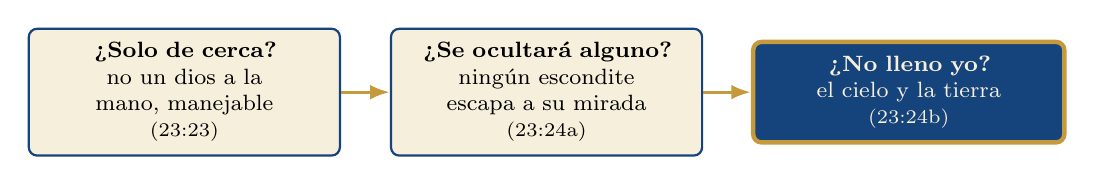
\begin{tikzpicture}[font=\footnotesize,
  caja/.style={draw=azul,line width=0.8pt,fill=papiro,rounded corners=3pt,inner sep=5pt,align=center,text width=3.6cm}]
 \node[caja] (a) at (0,0) {\textbf{¿Solo de cerca?}\\ no un dios a la mano, manejable\\ {\scriptsize(23:23)}};
 \node[caja] (b) at (4.6,0) {\textbf{¿Se ocultará alguno?}\\ ningún escondite escapa a su mirada\\ {\scriptsize(23:24a)}};
 \node[draw=dorado,line width=1.6pt,fill=azul,text=papiro,rounded corners=3pt,text width=3.6cm,align=center,inner sep=5pt] (c) at (9.2,0) {\textbf{¿No lleno yo?}\\ el cielo y la tierra\\ {\scriptsize(23:24b)}};
 \draw[-{Latex[length=2.5mm]},dorado,line width=1.2pt] (a)--(b); \draw[-{Latex[length=2.5mm]},dorado,line width=1.2pt] (b)--(c);
\end{tikzpicture}\par
{\footnotesize\color{gris}\textit{Figura 2.} El argumento de Jer 23:23--24. \textit{Nota.} Elaboración propia.}
\end{center}

Los falsos profetas trataban a Dios como a un dios de cerca: uno que se deja usar y que firma lo que el profeta ya ha decidido. Dios responde que también es ``Dios desde muy lejos'', el que está por encima de todo y al que nadie maneja. Y precisamente porque está por encima de todo, nada queda fuera de su alcance: ``¿Se ocultará alguno\ldots{} que yo no lo vea?''. MacArthur lo resume así: los falsos profetas no deben engañarse pensando que pueden esconder sus artimañas, porque Dios ``aquí se declara omnipresente y omnisciente, tanto en sentido inmanente como trascendente'' (MacArthur, 2011, nota a Jer 23:23).

\subsection{¿Cerca o lejos? Tres lecturas antiguas}

Desde la Antigüedad el versículo 23 se ha leído de maneras distintas:

\begin{center}\small\renewcommand{\arraystretch}{1.22}
\begin{tabular}{@{}L{2.6cm}L{5.6cm}L{6.0cm}@{}}
\toprule
\textbf{Texto} & \textbf{Lectura} & \textbf{Sentido} \\ \midrule
Texto masorético & pregunta: ``¿Soy yo Dios de cerca\ldots{} y no Dios desde muy lejos?'' & Dios no es solo cercano y manejable; también es el lejano, el que está por encima de todo. \\
Septuaginta & afirmación: \grc{θεὸς ἐγγίζων ἐγώ εἰμι, λέγει κύριος, καὶ οὐχὶ θεὸς πόρρωθεν}, ``Dios que se acerca soy yo, dice el Señor, y no Dios de lejos'' & Dios no está ausente: está cerca de los que obran en secreto. \\
Targum Jonatán & \heb{אֲנָא אֱלָהָא בְּרֵית עַלְמָא מִבְּרֵאשִׁית} y \heb{אֲנָא אֱלָהָא עֲתִידְנָא לְחַדָתָא עַלְמָא} & ``Yo soy el Dios que creé el mundo desde el principio\ldots{} yo soy el Dios que renovaré el mundo para los justos'': lo ``cercano'' y lo ``lejano'' se leen en el tiempo. \\
\bottomrule
\end{tabular}\par
{\footnotesize\color{gris}\textit{Tabla 2.} Jer 23:23 en tres textos antiguos. \textit{Nota.} Elaboración propia a partir de la BHS, Rahlfs-Hanhart (2006) y el Targum Jonatán (Sefaria); traducción propia.}
\end{center}

\begin{nota}[Precisión textual]
La Septuaginta convierte la pregunta en afirmación y, en apariencia, dice lo contrario: ``Dios que se acerca soy yo\ldots{} y no Dios de lejos''. Sin embargo, las dos lecturas llegan al mismo punto por caminos opuestos. El texto hebreo niega que Dios sea solo cercano y, por eso, manejable; la Septuaginta niega que sea lejano y, por eso, ciego. Aquí se sigue el texto hebreo, como hace la RVR1960. La lectura temporal del Targum es una interpretación judía antigua.
\end{nota}

\subsection{``¿No lleno yo el cielo y la tierra?''}

El verbo \heb{מָלֵא} \emph{male'} aparece en el hebreo bíblico ``unas 250 veces''. Vine observa que, en su uso transitivo, ``tiene el sentido de `llenar' todos los ámbitos, sin necesariamente `llenar' todos los espacios'' (Vine, 1999, ``Llenar''). En esa clave hay que leer Jer 23:24: Dios no ocupa el universo como el agua ocupa un vaso, por volumen o por partes, sino que está presente en todos sus ámbitos con todo su ser.

La misma raíz sostiene el canto de los serafines: ``Santo, santo, santo, \SENOR{} de los ejércitos; toda la tierra está llena de su gloria'' (Is 6:3), \heb{מְלֹא כָל־הָאָרֶץ כְּבוֹדוֹ}. El Targum Jonatán lee Jer 23:24 desde ese canto: \heb{הֲלָא יַת שְׁמַיָא וְיַת אַרְעָא יְקָרִי מְלֵי}, ``¿no llena \destacar{mi gloria} los cielos y la tierra?''. La Septuaginta, por su parte, traduce con el verbo que más tarde usará Pablo: \grc{μὴ οὐχὶ τὸν οὐρανὸν καὶ τὴν γῆν ἐγὼ πληρῶ;}.

\begin{nota}[Precisión]
El Targum añade ``mi gloria'' (\heb{יְקָרִי}) donde el hebreo dice ``yo''. Es su manera habitual de hablar de Dios con reverencia, sin atribuirle extensión física. La misma prudencia se observa en el Targum Ónkelos de Gn 28:16 (véase la sección~\ref{sec:judaismo-omni}).
\end{nota}

%===================================================================
\section{La palabra: el vocabulario de la presencia}

\subsection{Sin una palabra, con muchas}

El hebreo bíblico no dispone de un sustantivo abstracto para ``omnipresencia''. Nombra la presencia de Dios con palabras concretas: un rostro, un adverbio de lugar, una preposición, un adjetivo de cercanía, un verbo de llenar. Así habla de Dios la lengua de Israel, no por definiciones sino por relaciones.

\begin{center}
\begin{tikzpicture}[font=\footnotesize]
 \node[draw=dorado,line width=1.6pt,fill=azul,text=papiro,circle,minimum size=2.0cm,align=center] (c) at (0,0) {\textbf{La}\\\textbf{presencia}};
 \node[draw=azul,fill=papiro,rounded corners=3pt,text width=3.2cm,align=center,inner sep=4pt] (p) at (-5.0,1.7) {\heb{פָּנִים} \emph{panim}\\ rostro, presencia {\scriptsize(Éx 33:14)}};
 \node[draw=azul,fill=papiro,rounded corners=3pt,text width=3.2cm,align=center,inner sep=4pt] (s) at (0,2.6) {\heb{שָׁם} \emph{sham}\\ allí {\scriptsize(Sal 139:8)}};
 \node[draw=azul,fill=papiro,rounded corners=3pt,text width=3.2cm,align=center,inner sep=4pt] (i) at (5.0,1.7) {\heb{עִם} \emph{im}\\ con {\scriptsize(Gn 28:15)}};
 \node[draw=azul,fill=papiro,rounded corners=3pt,text width=3.2cm,align=center,inner sep=4pt] (q) at (-5.0,-1.7) {\heb{קָרוֹב} \emph{qarov}\\ cerca {\scriptsize(Sal 145:18)}};
 \node[draw=azul,fill=papiro,rounded corners=3pt,text width=3.2cm,align=center,inner sep=4pt] (m) at (0,-2.6) {\heb{מָקוֹם} \emph{maqom}\\ lugar {\scriptsize(Gn 28:16)}};
 \node[draw=azul,fill=papiro,rounded corners=3pt,text width=3.2cm,align=center,inner sep=4pt] (l) at (5.0,-1.7) {\heb{מָלֵא} \emph{male'}\\ llenar {\scriptsize(Jer 23:24)}};
 \foreach \n in {p,s,i,q,m,l}\draw[dorado,line width=1.1pt](c)--(\n);
\end{tikzpicture}\par
{\footnotesize\color{gris}\textit{Figura 3.} El vocabulario hebreo de la presencia de Dios. \textit{Nota.} Elaboración propia.}
\end{center}

\subsection{\emph{Panim}: el rostro que acompaña}

\heb{פָּנִים} \emph{panim} significa ``rostro, faz, cara''; aparece ``unas 2.100 veces'' y siempre en plural (Vine, 1999, ``Rostro''). Unido a preposiciones forma la expresión más frecuente de la presencia, \heb{לִפְנֵי יְהוָה} \emph{lifné Adonay}, ``delante del \SENOR{}''. Tras el becerro de oro, cuando Dios anuncia que no subirá en medio del pueblo, Moisés intercede y obtiene esta respuesta:

\hebverso{פָּנַי יֵלֵכוּ וַהֲנִחֹתִי לָךְ}
\begin{cita}Y él dijo: Mi presencia irá contigo, y te daré descanso. Y Moisés respondió: Si tu presencia no ha de ir conmigo, no nos saques de aquí.\fuente{(Éx 33:14--15)}\end{cita}

Literalmente, ``Mi rostro irá''. Moisés no pide un lugar; pide una compañía. Para Israel, la presencia de Dios no es en primer término una idea sobre el espacio, sino la seguridad de que Dios camina con su pueblo. Por eso el pan que permanecía siempre sobre la mesa del santuario se llamaba \heb{לֶחֶם הַפָּנִים}, ``pan del rostro'' (RVR1960: ``de la proposición''; Nm 4:7): pan puesto de continuo en la presencia de Dios.

\subsection{\emph{Sham}: ``allí estás tú''}

El adverbio \heb{שָׁם} \emph{sham}, ``allí'', es el eje del Salmo 139:7--12. El salmista imagina una por una todas las salidas posibles, y en cada una de ellas encuentra a Dios:

\hebverso{אָנָה אֵלֵךְ מֵרוּחֶךָ וְאָנָה מִפָּנֶיךָ אֶבְרָח\\ אִם־אֶסַּק שָׁמַיִם שָׁם אָתָּה וְאַצִּיעָה שְׁאוֹל הִנֶּךָּ}
\begin{cita}¿A dónde me iré de tu Espíritu? ¿Y a dónde huiré de tu presencia? Si subiere a los cielos, allí estás tú; Y si en el Seol hiciere mi estrado, he aquí, allí tú estás. Si tomare las alas del alba Y habitare en el extremo del mar, Aun allí me guiará tu mano, Y me asirá tu diestra. Si dijere: Ciertamente las tinieblas me encubrirán; Aun la noche resplandecerá alrededor de mí. Aun las tinieblas no encubren de ti, Y la noche resplandece como el día; Lo mismo te son las tinieblas que la luz.\fuente{(Sal 139:7--12)}\end{cita}

\begin{filologia}[Sal 139:7--12]
\begin{tabular}{@{}L{3.6cm}L{1.6cm}L{9.6cm}@{}}
\heb{מֵרוּחֶךָ} // \heb{מִפָּנֶיךָ} & \heb{רוח}, \heb{פנה} & ``de tu Espíritu'' // ``de tu rostro'': paralelismo sinónimo. El Espíritu de Dios es Dios presente (véase el capítulo ``Dios es Espíritu''). \\[2pt]
\heb{אֶבְרָח} \emph{evraj} & \heb{ברח} & ``huiré'': el mismo verbo de Jonás, que se levantó ``para huir'' (\heb{לִבְרֹחַ}) de delante del \SENOR{} (Jon 1:3). \\[2pt]
\heb{שָׁם אָתָּה} & --- & ``allí tú''. Sin verbo, como es normal en hebreo: la presencia se afirma sin necesidad de decir ``estás''. \\[2pt]
\heb{הִנֶּךָּ} \emph{hinneká} & --- & ``¡he aquí tú!'': una exclamación de hallazgo. En el Seol, el lugar de los muertos, el salmista se encuentra con Dios. \\[2pt]
\heb{כַנְפֵי־שָׁחַר} & \heb{שׁחר} & ``las alas del alba'': el extremo oriente, donde nace la luz; ``el extremo del mar'', el extremo occidente. \\[2pt]
\heb{גַּם־שָׁם} & --- & ``aun allí'': la mano que el fugitivo creía dejar atrás es la que lo ``guía'' y lo ``ase''. \\
\end{tabular}
\end{filologia}

Ni los cuatro extremos del mundo antiguo (arriba, abajo, oriente, occidente) ni la oscuridad ofrecen una salida. La Septuaginta traduce el final del versículo 8 con un verbo de presencia: \grc{ἐὰν καταβῶ εἰς τὸν ᾅδην, πάρει}, ``si bajo al Hades, estás presente'' (Sal 138:8 LXX). \grc{Πάρει} es la forma de \grc{πάρειμι}, ``estar presente''.

\begin{nota}[Precisión]
El Salmo 139 es el texto ancla del capítulo sobre la omnisciencia. Aquí se lee solo la segunda estrofa (vv.~7--12), que trata de la presencia. En el salmo las dos verdades caminan juntas: Dios conoce porque está, y está para conocer.
\end{nota}

Amós aplica el mismo esquema al juicio: ``Aunque cavasen hasta el Seol, de allá los tomará mi mano; y aunque subieren hasta el cielo, de allá los haré descender. Si se escondieren en la cumbre del Carmelo, allí los buscaré'' (Am 9:2--3). En los versículos 2 a 4 repite cinco veces \heb{מִשָּׁם}, ``de allí''. Lo que en el Salmo 139 es consuelo, en Amós se vuelve advertencia: la presencia es la misma, y lo que cambia es la relación con ella.

\subsection{\emph{Im} y \emph{qarov}: ``contigo'' y ``cerca''}

La preposición \heb{עִם} \emph{im} (``con'') y su sinónimo \heb{אֵת} \emph{et} sostienen la promesa más repetida de la Escritura: ``Yo estoy contigo''. Dios la dirige a Jacob, \heb{וְהִנֵּה אָנֹכִי עִמָּךְ}, ``He aquí, yo estoy contigo'' (Gn 28:15); a Israel en el exilio, ``Cuando pases por las aguas, yo estaré contigo (\heb{אִתְּךָ־אָנִי})'' (Is 43:2); y a Josué, ``\SENOR{} tu Dios estará contigo en dondequiera que vayas'' (Jos 1:9). De esta preposición nace el nombre \heb{עִמָּנוּאֵל}, ``con nosotros, Dios''.

El adjetivo \heb{קָרוֹב} \emph{qarov}, ``cercano'', dice lo mismo desde la experiencia de la oración:

\begin{cita}Porque ¿qué nación grande hay que tenga dioses tan cercanos a ellos como lo está \SENOR{} nuestro Dios en todo cuanto le pedimos?\fuente{(Dt 4:7)}\end{cita}
\begin{cita}Cercano está \SENOR{} a todos los que le invocan, A todos los que le invocan de veras.\fuente{(Sal 145:18)}\end{cita}

La cercanía bíblica no se reduce al espacio: es la cercanía de quien oye. Las naciones tenían dioses visibles y cercanos en sus santuarios; Israel tenía un Dios sin imagen y, precisamente por eso, más cercano, pues estaba en ``todo cuanto le pedimos''.

\subsection{\emph{Maqom} y \emph{kul}: el lugar que no lo contiene}

\heb{מָקוֹם} \emph{maqom}, ``lugar'', deriva de la raíz \heb{קום}, ``levantarse, estar en pie'': es el sitio donde algo está. La palabra resulta clave en Betel (Gn 28:11--19, seis veces) y en Pr 15:3: \heb{בְּכָל־מָקוֹם עֵינֵי יְהוָה צֹפוֹת רָעִים וְטוֹבִים}, ``Los ojos de \SENOR{} están en todo lugar, mirando a los malos y a los buenos''. Dios escogió un \emph{maqom} para su Nombre (Dt 12:5), pero ningún \emph{maqom} lo contiene. Salomón lo confesó con el verbo \heb{כּוּל} \emph{kul} en su forma intensiva, ``contener, abarcar'':

\hebverso{הִנֵּה הַשָּׁמַיִם וּשְׁמֵי הַשָּׁמַיִם לֹא יְכַלְכְּלוּךָ אַף כִּי־הַבַּיִת הַזֶּה אֲשֶׁר בָּנִיתִי}
\begin{cita}Pero ¿es verdad que Dios morará sobre la tierra? He aquí que los cielos, los cielos de los cielos, no te pueden contener; ¿cuánto menos esta casa que yo he edificado?\fuente{(1 R 8:27)}\end{cita}

``Los cielos de los cielos'' (\heb{שְׁמֵי הַשָּׁמַיִם}) es un superlativo: lo más alto que la mente puede concebir. Y, sin embargo, en esa misma oración Salomón pide que Dios oiga la súplica hecha ``en este lugar'' (8:30). La casa no contiene a Dios, pero Dios se compromete a escuchar allí. Esa tensión entre el Dios a quien nada contiene y el Dios que se deja hallar en un lugar recorre toda la Biblia y encuentra su resolución en Cristo.

\subsection{El espectro completo}

\begin{center}\small\renewcommand{\arraystretch}{1.18}
\begin{tabular}{@{}L{3.1cm}L{3.4cm}L{3.6cm}L{3.9cm}@{}}
\toprule
\textbf{Término} & \textbf{Sentido} & \textbf{LXX / NT} & \textbf{Textos} \\ \midrule
\heb{פָּנִים} \emph{panim} & rostro, presencia & \grc{πρόσωπον} & Éx 33:14; Sal 139:7; Jon 1:3; 2 Ts 1:9 \\
\heb{שָׁם} \emph{sham} & allí & \grc{ἐκεῖ} & Sal 139:8, 10; Am 9:2--3; Ez 48:35 \\
\heb{עִם} \emph{im}, \heb{אֵת} \emph{et} & con & \grc{μετά} & Gn 28:15; Is 43:2; Is 7:14; Mt 1:23; 28:20 \\
\heb{קָרוֹב} \emph{qarov} & cercano & \grc{ἐγγύς}, \grc{ἐγγίζω} & Dt 4:7; Sal 145:18; Flp 4:5; Stg 4:8 \\
\heb{מָקוֹם} \emph{maqom} & lugar & \grc{τόπος} & Gn 28:16; Pr 15:3; Éx 33:21 \\
\heb{מָלֵא} \emph{male'} & llenar, estar lleno & \grc{πληρόω}, \grc{πλήρωμα} & Is 6:3; Jer 23:24; Ef 1:23; 4:10 \\
\heb{כּוּל} \emph{kul} & contener, abarcar & \grc{ἀρκέω} (LXX 3 R 8:27) & 1 R 8:27; 2 Cr 2:6 \\
--- & estar presente & \grc{πάρειμι} & Sal 138:8 LXX \\
\heb{שָׁכַן} \emph{shajan} & habitar & \grc{σκηνόω}, \grc{ἐνοικέω} & Éx 25:8; Jn 1:14; 2 Co 6:16 \\
\bottomrule
\end{tabular}\par
{\footnotesize\color{gris}\textit{Tabla 3.} El espectro de la presencia en hebreo y griego. \textit{Nota.} Elaboración propia a partir de Vine (1999), la BHS, Rahlfs-Hanhart (2006) y NA28.}
\end{center}

\subsection{Del hebreo a Pablo}

Dos líneas de vocabulario pasan casi intactas del Antiguo Testamento al griego de Pablo: la del verbo ``llenar'' y la del adjetivo ``cerca''.

\begin{center}
\begin{tikzpicture}[font=\footnotesize,
  caja/.style={draw=azul,line width=0.8pt,fill=papiro,rounded corners=3pt,inner sep=5pt,align=center,text width=3.6cm}]
 \node[caja] (a1) at (0,1.4) {\textbf{Hebreo}\\ \heb{אֲנִי מָלֵא} ``yo lleno''\\ {\scriptsize(Jer 23:24)}};
 \node[caja] (b1) at (4.7,1.4) {\textbf{LXX}\\ \grc{ἐγὼ πληρῶ}\\ {\scriptsize(Jer 23:24)}};
 \node[draw=dorado,line width=1.4pt,fill=azul,text=papiro,rounded corners=3pt,text width=3.6cm,align=center,inner sep=5pt] (c1) at (9.4,1.4) {\textbf{Pablo}\\ \grc{ἵνα πληρώσῃ τὰ πάντα}\\ {\scriptsize(Ef 4:10)}};
 \node[caja] (a2) at (0,-0.9) {\textbf{Hebreo}\\ \heb{קָרוֹב יְהוָה} ``cercano está el \SENOR{}''\\ {\scriptsize(Sal 145:18)}};
 \node[caja] (b2) at (4.7,-0.9) {\textbf{LXX}\\ \grc{ἐγγὺς κύριος}\\ {\scriptsize(Sal 144:18)}};
 \node[draw=dorado,line width=1.4pt,fill=azul,text=papiro,rounded corners=3pt,text width=3.6cm,align=center,inner sep=5pt] (c2) at (9.4,-0.9) {\textbf{Pablo}\\ \grc{ὁ κύριος ἐγγύς}\\ {\scriptsize(Flp 4:5)}};
 \draw[-{Latex[length=2.5mm]},dorado,line width=1.2pt] (a1)--(b1); \draw[-{Latex[length=2.5mm]},dorado,line width=1.2pt] (b1)--(c1);
 \draw[-{Latex[length=2.5mm]},dorado,line width=1.2pt] (a2)--(b2); \draw[-{Latex[length=2.5mm]},dorado,line width=1.2pt] (b2)--(c2);
\end{tikzpicture}\par
{\footnotesize\color{gris}\textit{Figura 4.} Dos cadenas léxicas de la presencia: hebreo, Septuaginta y Pablo. \textit{Nota.} Elaboración propia; la relación con Pablo es un eco de vocabulario, estudiado en la sección~\ref{sec:cristo-omni}.}
\end{center}

%===================================================================
\section{El Nombre que revela la presencia}

\subsection{\SENOR{}-sama: ``el \SENOR{} está allí''}

El libro de Ezequiel se cierra con un nombre. El profeta había visto cómo la gloria del \SENOR{} abandonaba el templo profanado: ``se elevó de encima del umbral de la casa'' (Ez 10:18) y luego ``se elevó de en medio de la ciudad, y se puso sobre el monte que está al oriente'' (11:23). Más tarde la vio regresar: ``la gloria de \SENOR{} entró en la casa por la vía de la puerta que daba al oriente\ldots{} y he aquí que la gloria de \SENOR{} llenó la casa'' (43:4--5). Y al final, cuando describe la ciudad restaurada, le da un nombre nuevo:

\hebverso{וְשֵׁם־הָעִיר מִיּוֹם יְהוָה שָׁמָּה}
\begin{cita}En derredor tendrá dieciocho mil cañas. Y el nombre de la ciudad desde aquel día será \SENOR{}-sama.\fuente{(Ez 48:35)}\end{cita}

\begin{filologia}[Ez 48:35]
\begin{tabular}{@{}L{3.6cm}L{1.6cm}L{9.6cm}@{}}
\heb{וְשֵׁם־הָעִיר} & \heb{שׁם} & ``y el nombre de la ciudad''. Jerusalén no se nombra: la ciudad recibe su identidad de quien la habita. \\[2pt]
\heb{מִיּוֹם} & \heb{יום} & ``desde (aquel) día'': un nombre que empieza en el día de la restauración y ya no cambia. \\[2pt]
\heb{יְהוָה שָׁמָּה} \emph{Adonay shammá} & \heb{שׁם} & ``el \SENOR{} (está) allí''. \heb{שָׁמָּה} es \heb{שָׁם} con la terminación \heb{־ָה} de dirección o de énfasis. Hay un juego de sonido entre \heb{שֵׁם} (\emph{shem}, ``nombre'') y \heb{שָׁמָּה} (\emph{shammá}, ``allí''). \\[2pt]
Targum Jonatán & --- & \heb{מִיוֹמָא דִי יִשְׁרֵי יְיָ שְׁכִנְתֵּיהּ תַּמָן}: ``desde el día en que el \SENOR{} haga reposar su Shejiná allí''. \\
\end{tabular}
\end{filologia}

\begin{nota}[Precisión textual]
La Septuaginta no traduce el nombre: dice \grc{καὶ τὸ ὄνομα τῆς πόλεως ἀφ’ ἧς ἂν ἡμέρας γένηται, ἔσται τὸ ὄνομα αὐτῆς}, ``y el nombre de la ciudad, desde el día en que sea, será su nombre''. Todo indica que leyó las consonantes \heb{שמה} como \emph{shemáh}, ``su nombre'', y no como \emph{shammá}, ``allí''. Aquí se sigue el texto hebreo. La partida y el regreso de la gloria se estudian en el capítulo de la conclusión, ``La gloria de Dios''.
\end{nota}

El último versículo de Ezequiel no promete que la ciudad será grande, rica o segura; promete que Dios estará allí. MacArthur lo llama ``la consumación de la historia de Israel: ¡el regreso de la presencia de Dios!'' (MacArthur, 2011, nota a Ez 48:35). El Dios que llena el cielo y la tierra no se conforma con estar en todas partes: quiere estar \destacar{con} su pueblo.

\subsection{Emanuel: ``Dios con nosotros''}

El segundo nombre vincula la presencia con una persona:

\hebverso{הִנֵּה הָעַלְמָה הָרָה וְיֹלֶדֶת בֵּן וְקָרָאת שְׁמוֹ עִמָּנוּ אֵל}
\begin{cita}Por tanto, el Señor mismo os dará señal: He aquí que la virgen concebirá, y dará a luz un hijo, y llamará su nombre Emanuel.\fuente{(Is 7:14)}\end{cita}

En el capítulo siguiente el nombre reaparece como grito de confianza frente a la invasión asiria: ``y extendiendo sus alas, llenará la anchura de tu tierra, oh Emanuel'' (Is 8:8); ``Tomad consejo, y será anulado\ldots{} porque Dios está con nosotros'' (\heb{כִּי עִמָּנוּ אֵל}, 8:10). Mateo lo lee cumplido en Jesús y lo traduce para sus lectores: \grc{Ἐμμανουήλ, ὅ ἐστιν μεθερμηνευόμενον μεθ’ ἡμῶν ὁ θεός}, ``Emanuel, que traducido es: Dios con nosotros'' (Mt 1:23).

\begin{nota}[Precisión]
El cumplimiento de Is 7:14 es objeto de discusión. La señal se dio a Acaz en su propio tiempo (7:16), y la palabra \heb{עַלְמָה} significa ``joven en edad de casarse''; la Septuaginta la tradujo \grc{παρθένος}, ``virgen'', y Mateo cita esa traducción. La lectura cristiana ve en Jesús el cumplimiento pleno de la señal, y es la que sigue esta serie.
\end{nota}

\subsection{Nombres y declaraciones de la presencia}

\begin{center}\small\renewcommand{\arraystretch}{1.2}
\begin{tabular}{@{}L{4.6cm}L{5.0cm}L{4.4cm}@{}}
\toprule
\textbf{Nombre o declaración} & \textbf{Original} & \textbf{Texto} \\ \midrule
\SENOR{}-sama, ``el \SENOR{} está allí'' & \heb{יְהוָה שָׁמָּה} & Ez 48:35 \\
Emanuel, ``Dios con nosotros'' & \heb{עִמָּנוּאֵל}; \grc{μεθ’ ἡμῶν ὁ θεός} & Is 7:14; 8:10; Mt 1:23 \\
Dios de cerca y Dios de lejos & \heb{אֱלֹהֵי מִקָּרֹב}\ldots{} \heb{אֱלֹהֵי מֵרָחֹק} & Jer 23:23 \\
Dios arriba en el cielo y abajo en la tierra & \heb{בַּשָּׁמַיִם מִמַּעַל וְעַל־הָאָרֶץ מִתָּחַת} & Dt 4:39; Jos 2:11 \\
El Alto y Sublime que habita con el humilde & \heb{מָרוֹם וְקָדוֹשׁ אֶשְׁכּוֹן וְאֶת־דַּכָּא} & Is 57:15 \\
El Dios de Bet-el & \heb{הָאֵל בֵּית־אֵל} & Gn 31:13 \\
``El Señor está cerca'' & \grc{ὁ κύριος ἐγγύς} & Flp 4:5 \\
\emph{HaMaqom}, ``el Lugar'' (nombre rabínico) & \heb{הַמָּקוֹם} & Bereshit Rabá 68:9 \\
\bottomrule
\end{tabular}\par
{\footnotesize\color{gris}\textit{Tabla 4.} Nombres y declaraciones que revelan la presencia de Dios. \textit{Nota.} Elaboración propia; \emph{HaMaqom} no es un nombre bíblico, sino de la literatura rabínica.}
\end{center}

\begin{nota}[Precisión]
En esta serie, el Nombre que revela el atributo es \SENOR{}-sama (Ez 48:35), y su cumplimiento personal es Emanuel (Is 7:14; Mt 1:23). Se trata de un nombre de lugar: no afirma ``Dios está en todas partes'', sino ``Dios está allí'', en medio de su pueblo. En la Biblia, la omnipresencia de Dios nunca es una presencia indiferente; es la presencia de quien se compromete.
\end{nota}

%===================================================================
\section{Definición}

\subsection{¿Qué es la omnipresencia de Dios?}

\begin{tcolorbox}[colback=papiro,colframe=azul,boxrule=1pt,arc=3pt,title={Definición},colbacktitle=azul,coltitle=papiro]
La omnipresencia es la perfección eterna de Dios por la cual él, sin ser contenido ni limitado por ningún lugar, está presente con todo su ser en todo lugar: llena el cielo y la tierra, sostiene y ve todas las cosas, y se hace presente de manera especial para habitar con su pueblo, para juzgar al pecador y, en plenitud, en el Hijo hecho carne.
\end{tcolorbox}
{\footnotesize\color{gris}Definición de síntesis de esta serie, a partir de los textos estudiados.}\medskip

\begin{center}\small\renewcommand{\arraystretch}{1.2}
\begin{tabular}{@{}L{3.6cm}L{10.4cm}@{}}
\toprule
\textbf{Rasgo} & \textbf{Texto} \\ \midrule
No contenido & ``los cielos de los cielos, no te pueden contener'' (1 R 8:27) \\
Presente en todo lugar & ``¿No lleno yo\ldots{} el cielo y la tierra?'' (Jer 23:24) \\
Con todo su ser & ``¿A dónde huiré de tu presencia? Si subiere a los cielos, allí estás tú'' (Sal 139:7--8) \\
Que sostiene & ``en él vivimos, y nos movemos, y somos'' (Hch 17:28) \\
Que ve & ``Los ojos de \SENOR{} están en todo lugar'' (Pr 15:3) \\
Trascendente y cercano & ``Yo habito en la altura y la santidad, y con el quebrantado y humilde de espíritu'' (Is 57:15) \\
Que se compromete & ``He aquí, yo estoy contigo, y te guardaré por dondequiera que fueres'' (Gn 28:15) \\
\bottomrule
\end{tabular}\par
{\footnotesize\color{gris}\textit{Tabla 5.} Rasgos de la omnipresencia. \textit{Nota.} Elaboración propia.}
\end{center}

\subsection{Inmensidad y omnipresencia}

La teología distingue en esta perfección dos caras. La \destacar{inmensidad} afirma que ningún espacio contiene ni limita a Dios, que está por encima de toda medida (1 R 8:27; Is 40:12). La \destacar{omnipresencia} añade que, sin estar limitado por el espacio, Dios está presente en cada lugar con todo su ser (Jer 23:24; Sal 139:7--8). Berkhof define la inmensidad como la perfección por la cual Dios trasciende toda limitación espacial y, sin embargo, está presente en cada punto del espacio con todo su ser (Berkhof, 1938). La primera mira hacia arriba, a Dios sobre el mundo; la segunda mira hacia dentro, a Dios en el mundo. Ambas son necesarias: sin inmensidad, Dios sería una parte del mundo; sin omnipresencia, le sería ajeno.

\begin{center}
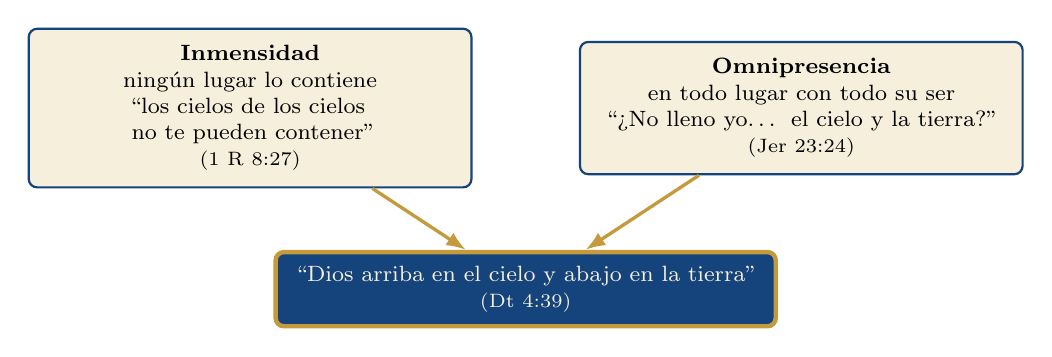
\begin{tikzpicture}[font=\footnotesize]
 \node[draw=azul,line width=0.8pt,fill=papiro,rounded corners=3pt,text width=5.2cm,align=center,inner sep=6pt] (i) at (0,0) {\textbf{Inmensidad}\\ ningún lugar lo contiene\\ ``los cielos de los cielos no te pueden contener''\\ {\scriptsize(1 R 8:27)}};
 \node[draw=azul,line width=0.8pt,fill=papiro,rounded corners=3pt,text width=5.2cm,align=center,inner sep=6pt] (o) at (7.0,0) {\textbf{Omnipresencia}\\ en todo lugar con todo su ser\\ ``¿No lleno yo\ldots{} el cielo y la tierra?''\\ {\scriptsize(Jer 23:24)}};
 \node[draw=dorado,line width=1.6pt,fill=azul,text=papiro,rounded corners=3pt,text width=6.0cm,align=center,inner sep=5pt] (s) at (3.5,-2.3) {``Dios arriba en el cielo y abajo en la tierra''\\ {\scriptsize(Dt 4:39)}};
 \draw[-{Latex[length=2.5mm]},dorado,line width=1.2pt](i)--(s); \draw[-{Latex[length=2.5mm]},dorado,line width=1.2pt](o)--(s);
\end{tikzpicture}\par
{\footnotesize\color{gris}\textit{Figura 5.} Las dos caras de la perfección. \textit{Nota.} Elaboración propia a partir de Berkhof (1938).}
\end{center}

\subsection{Una presencia, varios modos}

En cuanto a su ser, Dios no está ``más'' en un lugar que en otro. La Escritura, sin embargo, distingue diversas maneras en que se hace presente, según la relación que guarda con sus criaturas.

\begin{center}\small\renewcommand{\arraystretch}{1.2}
\begin{tabular}{@{}L{3.2cm}L{6.0cm}L{4.8cm}@{}}
\toprule
\textbf{Modo} & \textbf{Qué hace Dios} & \textbf{Textos} \\ \midrule
Sustentadora & da y mantiene la existencia de todo & Neh 9:6; Hch 17:28; Col 1:17 \\
Que ve y juzga & mira a malos y buenos; nadie escapa & Pr 15:3; Am 9:2--4; He 4:13 \\
De pacto & habita en medio de Israel, en el tabernáculo y el templo & Éx 25:8; 29:45; Lv 26:11--12 \\
De gracia & habita en el creyente y en la iglesia por su Espíritu & Jn 14:23; 1 Co 3:16; Ef 2:22 \\
Encarnada & ``el Verbo fue hecho carne, y habitó entre nosotros'' & Jn 1:14; Col 2:9 \\
Gloriosa & el tabernáculo de Dios con los hombres; verán su rostro & Ap 21:3; 22:4; Sal 16:11 \\
\bottomrule
\end{tabular}\par
{\footnotesize\color{gris}\textit{Tabla 6.} Los modos de la presencia de Dios. \textit{Nota.} Elaboración propia; la clasificación es una síntesis teológica, no una lista bíblica.}
\end{center}

\subsection{Lo que no significa}

\begin{center}\small\renewcommand{\arraystretch}{1.22}
\begin{tabular}{@{}L{4.0cm}L{10.0cm}@{}}
\toprule
\textbf{Malentendido} & \textbf{Respuesta bíblica} \\ \midrule
``Dios es todo'' (panteísmo) & Dios llena el mundo, pero no es el mundo: ``El cielo es mi trono, y la tierra estrado de mis pies\ldots{} Mi mano hizo todas estas cosas'' (Is 66:1--2). \\
Un pedazo de Dios en cada lugar & ``La omnipresencia no significa que una parte de Dios está en China y otra parte está en Inglaterra, sino que Dios está en todo lugar al mismo tiempo'' (Washer, 2021, p. 89). \\
Una sustancia extendida & Dios es Espíritu y no tiene cuerpo: ``precisamente porque es `espíritu', llena el cielo y la tierra'' (Pink, 2020, cap. 16, p. 83). \\
Indiferencia moral & Está en todo lugar, pero no aprueba todo: ``vuestras iniquidades han hecho división entre vosotros y vuestro Dios'' (Is 59:2). \\
Todos gozan de su presencia & Hay una presencia que bendice y una que juzga; el impío será ``excluido de la presencia del Señor'' (2 Ts 1:9). \\
Los lugares no importan & Dios eligió lugares para encontrarse con su pueblo (Gn 28:17; Dt 12:5; 1 R 8:29--30); en Cristo, el lugar es una persona (Jn 2:21). \\
\bottomrule
\end{tabular}\par
{\footnotesize\color{gris}\textit{Tabla 7.} Lo que la omnipresencia no significa. \textit{Nota.} Elaboración propia.}
\end{center}

\subsection{Trascendente y cercano}

Isaías reúne las dos caras en una sola frase:

\hebverso{מָרוֹם וְקָדוֹשׁ אֶשְׁכּוֹן וְאֶת־דַּכָּא וּשְׁפַל־רוּחַ}
\begin{cita}Porque así dijo el Alto y Sublime, el que habita la eternidad, y cuyo nombre es el Santo: Yo habito en la altura y la santidad, y con el quebrantado y humilde de espíritu, para hacer vivir el espíritu de los humildes, y para vivificar el corazón de los quebrantados.\fuente{(Is 57:15)}\end{cita}

Un mismo verbo, \heb{שָׁכַן} \emph{shajan}, ``habitar'', sirve para la altura y para el corazón quebrantado. Es el verbo del que procede el nombre del tabernáculo (\heb{מִשְׁכָּן}) y, en la tradición judía posterior, el de la Shejiná (\heb{שְׁכִינָה}). El salmista lo canta con asombro: ``¿Quién como \SENOR{} nuestro Dios, que se sienta en las alturas, que se humilla a mirar en el cielo y en la tierra?'' (Sal 113:5--6).

%===================================================================
\section{Teología: el Dios que llena el cielo y la tierra}

\subsection{Presente porque es Espíritu}

Junto al pozo de Sicar, la samaritana planteó a Jesús la cuestión de los lugares: ¿se adora en el monte Gerizim o en Jerusalén? Jesús lleva la pregunta a su raíz: ``Dios es Espíritu; y los que le adoran, en espíritu y en verdad es necesario que adoren'' (Jn 4:24). De allí nace la omnipresencia. Un ser con cuerpo ocupa un lugar y, al ocuparlo, deja libres todos los demás; Dios, que no tiene cuerpo, no ocupa los lugares, sino que los llena. Por eso el salmista pone en paralelo ``tu Espíritu'' y ``tu presencia'' (Sal 139:7): huir del Espíritu de Dios equivale a huir de su rostro, y ninguna de las dos huidas es posible. Como observa Pink (2020, cap. 16, p. 83), ``si Dios tuviera un cuerpo tangible, no sería omnipresente, estaría limitado a un lugar; pero precisamente porque es `espíritu', llena el cielo y la tierra''. Y lo que vale para su ser vale para todas sus perfecciones: ``Todo acerca de Dios es infinito. Su esencia llena el cielo y la tierra'' (cap. 16, p. 86).

Agustín abre sus \emph{Confesiones} con la misma pregunta de Jer 23:24: \emph{Capiunt ergone te caelum et terra, quoniam tu imples ea? An imples et restat, quoniam non te capiunt?}, ``¿Te contienen, pues, el cielo y la tierra, porque tú los llenas? ¿O los llenas, y sobra algo de ti, porque no te contienen?'' (Agustín, \emph{Confesiones} I, 3, 3; traducción propia). Su reflexión concluye preguntando si Dios no está, más bien, todo entero en todas partes, sin que nada lo contenga entero. Es, en el fondo, la pregunta de Salomón al dedicar el templo: ``He aquí que los cielos, los cielos de los cielos, no te pueden contener; ¿cuánto menos esta casa que yo he edificado?'' (1 R 8:27).

\subsection{Inmenso, eterno y todopoderoso}

La presencia de Dios no es una perfección aislada. La Escritura la une a su eternidad y a su poder, y la tradición ha sabido verlo. Charnock lo condensa en una frase que recorre las tres medidas de la criatura: ``Como su esencia es inmensa, no puede ser confinada en un lugar; como es eterno, no puede medirse en el tiempo; así que como es todopoderoso, no puede ser limitado en lo que respecta a la acción'' (citado en Pink, 2020, cap. 9, p. 47). Lo que el tiempo no mide y la acción no limita, tampoco lo encierra el espacio. En esa misma línea Berkhof distingue la inmensidad (Dios sobre el espacio) de la omnipresencia (Dios en cada punto del espacio con todo su ser) (Berkhof, 1938).

El libro de Job hace sentir esa inmensidad desde la altura: ``¿No está Dios en la altura de los cielos? Mira lo encumbrado de las estrellas, cuán elevadas están'' (Job 22:12). La frase que sigue, ``por el circuito del cielo se pasea'' (22:14), se ha leído como una imagen de ``la inmensidad de su presencia'' (Pink, 2020, cap. 9, p. 48).

\begin{nota}[Precisión]
En su contexto, Elifaz atribuye a Job la idea de que la altura aleja a Dios: ``¿Qué sabe Dios? ¿Cómo juzgará a través de la oscuridad? Las nubes le rodearon, y no ve'' (Job 22:13--14). Leer 22:14 como imagen de la inmensidad es, por tanto, una lectura teológica; el texto mismo exhibe el error contrario, el de quien confunde la altura de Dios con su lejanía. A ese error responde Jeremías: Dios es a la vez ``de cerca'' y ``desde muy lejos'' (Jer 23:23).
\end{nota}

\subsection{La presencia del Rey}

La presencia bíblica no es un ambiente difuso ni una energía repartida por el mundo, sino la presencia de un Rey. ``El cielo es mi trono, y la tierra estrado de mis pies'' (Is 66:1): el mismo texto que niega que una casa pueda contener a Dios presenta el universo entero como la sala de su trono. El salmista lo canta: ``\SENOR{} estableció en los cielos su trono, y su reino domina sobre todos'' (Sal 103:19). Llenar el cielo y la tierra es gobernarlos. De ahí la advertencia de Spurgeon: ``los hombres permitirán que Dios esté en todas partes, excepto en su Trono'' (citado en Pink, 2020, cap. 6, p. 30). Muchos aceptan un Dios presente en todas partes con tal de que no mande en ninguna. Pero una omnipresencia sin trono no pasa de ser una idea vaga; la que enseña la Escritura es la del Señor que está en todo lugar porque todo lugar le pertenece.

\subsection{La presencia que ve}

La presencia de Dios es también mirada. Jeremías reúne ambas cosas en una sola pregunta: ``¿Se ocultará alguno, dice \SENOR{}, en escondrijos que yo no lo vea?'' (Jer 23:24). Proverbios lo formula como sentencia: ``Los ojos de \SENOR{} están en todo lugar, mirando a los malos y a los buenos'' (Pr 15:3). Omnipresencia y omnisciencia son dos lados de una misma verdad: Dios conoce porque está, y está para conocer. De esa verdad se sigue una consecuencia moral, que Pink expresa con una exclamación: ``¡Qué freno sería para nosotros si meditáramos en ello con más frecuencia!'' (Pink, 2020, cap. 3, p. 19). Se sigue también una doble consecuencia pastoral, que Washer señala así: ``Para el cristiano, la omnipresencia de Dios infunde gran confianza y consuelo; cada creyente, desde el más grande hasta el más pequeño, se beneficia de la presencia indivisa de Dios. Para el incrédulo, la omnipresencia de Dios infunde terror porque no hay ninguna posibilidad de esconderse o escapar de Su presencia'' (Washer, 2021, p. 89).

Esa doble consecuencia ya está presente en el Salmo 139. El salmista que pregunta ``¿a dónde huiré de tu presencia?'' (Sal 139:7) acaba diciendo ``aun allí me guiará tu mano, y me asirá tu diestra'' (139:10). La presencia que impide la fuga es la misma que sostiene. Frente a ella la mente queda sobrepasada, como reconoce Pink al contemplar la eternidad, la inmaterialidad, la omnipresencia y el poder de Dios: ``nuestras mentes quedan abrumadas'' (Pink, 2020, cap. 19, p. 99). El salmista, con todo, no se detiene en el asombro, sino que lo transforma en confianza y en oración (139:23--24).

\begin{center}\small\renewcommand{\arraystretch}{1.22}
\begin{tabular}{@{}L{2.6cm}L{4.4cm}L{7.0cm}@{}}
\toprule
\textbf{Unida a} & \textbf{Texto} & \textbf{Lo que muestra} \\ \midrule
Espíritu & Jn 4:24; Sal 139:7 & Dios no ocupa un lugar: los llena, porque no tiene cuerpo. \\
Inmensidad & 1 R 8:27; Jer 23:24 & Ningún espacio lo contiene, y está entero en cada lugar. \\
Eternidad y poder & Jer 23:23; Job 22:12 & Lo que el tiempo no mide y la acción no limita, el espacio no lo encierra. \\
Soberanía & Is 66:1; Sal 103:19 & Está en todo lugar como Rey: llenar es gobernar. \\
Saber & Pr 15:3; Jer 23:24 & La presencia es mirada: no hay escondite delante de él. \\
Cercanía & Sal 139:10; Is 57:15 & La presencia que impide huir es la que guía y sostiene. \\
\bottomrule
\end{tabular}\par
{\footnotesize\color{gris}\textit{Tabla 8.} La omnipresencia unida a otras perfecciones. \textit{Nota.} Elaboración propia; textos de la RVR1960.}
\end{center}

\subsection{Preguntas que plantea la Escritura}

\emph{¿Por qué decimos ``Padre nuestro que estás en los cielos''?} Porque el cielo es el lugar del trono, desde donde Dios gobierna y donde su gloria se manifiesta sin velo. Salomón pide que Dios oiga ``en los cielos, en el lugar de tu morada'' (1 R 8:30, 39) en la misma oración en que confiesa que los cielos no lo contienen (8:27). La expresión ``en los cielos'' señala la majestad de Dios, no su límite. Por eso aconseja el Predicador: ``Dios está en el cielo, y tú sobre la tierra; por tanto, sean pocas tus palabras'' (Ec 5:2).

\emph{¿Está Dios en el Seol?} El salmista responde que sí: ``si en el Seol hiciere mi estrado, he aquí, allí tú estás'' (Sal 139:8). Pablo, por su parte, habla de quienes serán ``excluidos de la presencia del Señor'' (2 Ts 1:9). No hay contradicción entre ambos textos. Dios está presente en todo lugar con su ser y con su juicio, pero existe una presencia de favor, de comunión y de gloria que el impío pierde. Isaías lo explica: el pecado no aleja a Dios en el espacio, sino que ``ha hecho ocultar de vosotros su rostro para no oír'' (Is 59:2).

\begin{nota}[Precisión]
La autoría paulina de 2 Tesalonicenses se discute. Con todo, la idea de una presencia que juzga y otra que bendice aparece también en el Antiguo Testamento (Am 9:2--4 frente a Sal 139:10) y en cartas indiscutidas de Pablo (Ro 2:5--8).
\end{nota}

\emph{Si Dios está en todas partes, ¿por qué buscarlo?} Porque la omnipresencia no equivale a comunión. Dios ``no está lejos de cada uno de nosotros'' (Hch 17:27) y, sin embargo, manda buscarlo: ``me buscaréis y me hallaréis, porque me buscaréis de todo vuestro corazón'' (Jer 29:13). Santiago lo expresa con el vocabulario de la cercanía: ``Acercaos a Dios, y él se acercará a vosotros'' (Stg 4:8).

%===================================================================
\section{Un encuentro en la historia de Israel: Betel}

\subsection{Un fugitivo en ``un cierto lugar''}

Jacob huye. Ha engañado a su padre y robado la bendición de su hermano, y Esaú ha jurado matarlo (Gn 27:41). Rebeca lo manda lejos: ``levántate y huye a casa de Labán mi hermano en Harán'' (27:43). Deja Beerseba, la tierra de Abraham e Isaac, y emprende el camino hacia el norte. Cuando el sol se pone, se detiene donde puede:

\hebverso{וַיִּפְגַּע בַּמָּקוֹם וַיָּלֶן שָׁם כִּי־בָא הַשֶּׁמֶשׁ}
\begin{cita}Salió, pues, Jacob de Beerseba, y fue a Harán. Y llegó a un cierto lugar, y durmió allí, porque ya el sol se había puesto; y tomó de las piedras de aquel paraje y puso a su cabecera, y se acostó en aquel lugar.\fuente{(Gn 28:10--11)}\end{cita}

El narrador calla qué lugar era; en un solo versículo lo llama tres veces ``el lugar'' (\heb{הַמָּקוֹם}). Jacob no busca a Dios, sino un sitio donde dormir.

\subsection{La escalera y la promesa}

\begin{cita}Y soñó: y he aquí una escalera que estaba apoyada en tierra, y su extremo tocaba en el cielo; y he aquí ángeles de Dios que subían y descendían por ella. Y he aquí, \SENOR{} estaba en lo alto de ella, el cual dijo: Yo soy \SENOR{}, el Dios de Abraham tu padre, y el Dios de Isaac; la tierra en que estás acostado te la daré a ti y a tu descendencia\ldots{} He aquí, yo estoy contigo, y te guardaré por dondequiera que fueres, y volveré a traerte a esta tierra; porque no te dejaré hasta que haya hecho lo que te he dicho.\fuente{(Gn 28:12--13, 15)}\end{cita}

\hebverso{אָכֵן יֵשׁ יְהוָה בַּמָּקוֹם הַזֶּה וְאָנֹכִי לֹא יָדָעְתִּי}
\begin{cita}Y despertó Jacob de su sueño, y dijo: Ciertamente \SENOR{} está en este lugar, y yo no lo sabía. Y tuvo miedo, y dijo: ¡Cuán terrible es este lugar! No es otra cosa que casa de Dios, y puerta del cielo.\fuente{(Gn 28:16--17)}\end{cita}

\begin{filologia}[Gn 28:11--17]
\begin{tabular}{@{}L{3.6cm}L{1.6cm}L{9.6cm}@{}}
\heb{וַיִּפְגַּע בַּמָּקוֹם} & \heb{פגע} & ``y llegó (dio) con el lugar''. \emph{Paga'} es ``topar, encontrarse con''. El artículo (``\emph{el} lugar'') anticipa que no es un sitio cualquiera. \\[2pt]
\heb{סֻלָּם} \emph{sullam} & \heb{סלל} & ``escalera'' o ``rampa''. Palabra que aparece solo aquí en la Biblia; la raíz significa ``amontonar, levantar un terraplén''. \\[2pt]
\heb{מֻצָּב}\ldots{} \heb{נִצָּב}\ldots{} \heb{מַצֵּבָה} & \heb{נצב} & La escalera está ``apoyada'' (\emph{mutsav}, 28:12), el \SENOR{} ``estaba'' (\emph{nitsav}, 28:13) y Jacob levanta una ``señal'' o estela (\emph{matsevá}, 28:18). Tres palabras de la misma raíz, ``estar firme, erguido''. \\[2pt]
\heb{עָלָיו} \emph{alav} & --- & ``sobre ella'' (la escalera) o ``junto a él'' (Jacob). La RVR1960 traduce ``en lo alto de ella''. \\[2pt]
\heb{אָנֹכִי עִמָּךְ} & --- & ``yo (estoy) contigo''. La promesa no está ligada al lugar: ``por dondequiera que fueres'' (\heb{בְּכֹל אֲשֶׁר־תֵּלֵךְ}). \\[2pt]
\heb{אָכֵן יֵשׁ יְהוָה} & --- & ``ciertamente hay \SENOR{}'': \heb{יֵשׁ} afirma existencia y presencia. \heb{אָכֵן} expresa la sorpresa de quien descubre algo que no esperaba. \\[2pt]
\heb{נוֹרָא} \emph{norá} & \heb{ירא} & ``temible'', de la misma raíz que ``tuvo miedo'' (\heb{וַיִּירָא}). La presencia descubierta produce reverencia. \\[2pt]
\heb{בֵּית אֱלֹהִים}, \heb{שַׁעַר הַשָּׁמָיִם} & --- & ``casa de Dios'' y ``puerta del cielo''. De aquí el nombre \heb{בֵּית־אֵל}, Bet-el (28:19). \\
\end{tabular}
\end{filologia}

\begin{nota}[Precisión]
La traducción de \heb{עָלָיו} es ambigua: puede significar ``sobre ella'' (la escalera) o ``junto a él'' (Jacob). La segunda lectura acentúa la cercanía, pues el \SENOR{} no estaría solo en lo alto, sino junto al que duerme. Ambas son gramaticalmente posibles, y la RVR1960 sigue la primera.
\end{nota}

\subsection{Seis veces ``lugar''}

La palabra \heb{מָקוֹם} aparece seis veces en Gn 28:11--19 (conteo propio en la BHS): tres en el versículo 11 y una en cada uno de los versículos 16, 17 y 19. El relato avanza así de ``un cierto lugar'' a ``este lugar'' donde está el \SENOR{}, y de allí a un lugar que recibe nombre.

\begin{center}
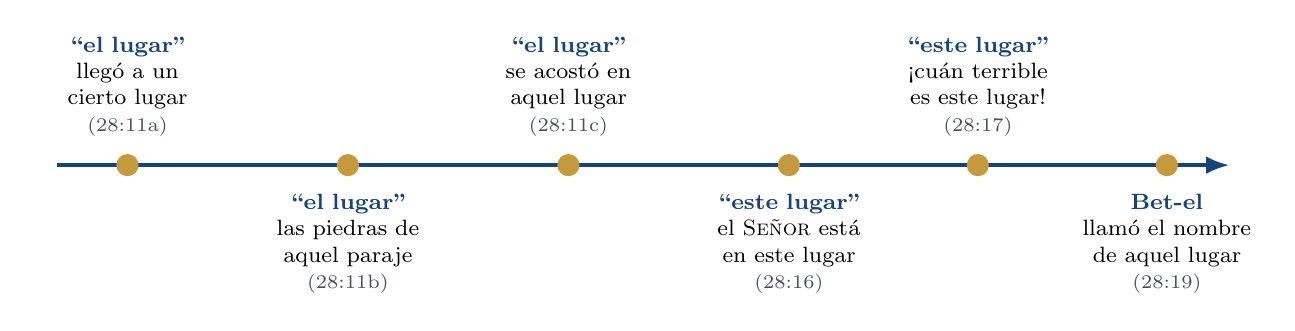
\begin{tikzpicture}[font=\footnotesize]
 \draw[line width=1.6pt,azul,-{Latex[length=3mm]}] (-0.3,0) -- (14.6,0);
 \foreach \x/\t/\b/\r/\pos in {0.6/{``el lugar''}/{llegó a un cierto lugar}/{28:11a}/above,
   3.4/{``el lugar''}/{las piedras de aquel paraje}/{28:11b}/below,
   6.2/{``el lugar''}/{se acostó en aquel lugar}/{28:11c}/above,
   9.0/{``este lugar''}/{el \SENOR{} está en este lugar}/{28:16}/below,
   11.4/{``este lugar''}/{¡cuán terrible es este lugar!}/{28:17}/above,
   13.8/{Bet-el}/{llamó el nombre de aquel lugar}/{28:19}/below}{
  \fill[dorado] (\x,0) circle (4pt);
  \node[\pos=7pt,text width=2.3cm,align=center] at (\x,0) {\textbf{\textcolor{azul}{\t}}\\ \b\\ {\scriptsize\color{gris}(\r)}};}
\end{tikzpicture}\par
{\footnotesize\color{gris}\textit{Figura 6.} \heb{מָקוֹם} en Gn 28:11--19. \textit{Nota.} Elaboración propia; conteo propio en la BHS.}
\end{center}

\subsection{``Y yo no lo sabía''}

Lo que Jacob descubre no es que Dios esté en Betel y en ninguna otra parte, sino que estaba donde él no lo esperaba. Había salido de la tierra de sus padres de noche, solo, con una piedra por almohada, y quizá pensaba que dejaba atrás, junto con la tienda de su padre, al Dios de Abraham e Isaac. El texto no revela lo que pensaba; registra lo que confesó: ``yo no lo sabía''. Matthew Henry extrae de allí la lección: ``Doquiera estemos, en la ciudad o en el desierto, en la casa o en el campo, en la tienda o en la calle, podemos mantener nuestra relación con el Cielo'' (Henry, 1999, Gn 28:16--19).

Tampoco la promesa queda confinada a Betel. El Dios que se reveló allí acompaña a Jacob durante veinte años en Harán (Gn 31:41), y en Harán mismo, lejos de Betel, le habla: ``Yo soy el Dios de Bet-el, donde tú ungiste la piedra, y donde me hiciste un voto'' (31:13). El ``Dios de Bet-el'' habla en Harán: su nombre evoca un lugar, pero él no está atado a ese lugar.

\begin{center}
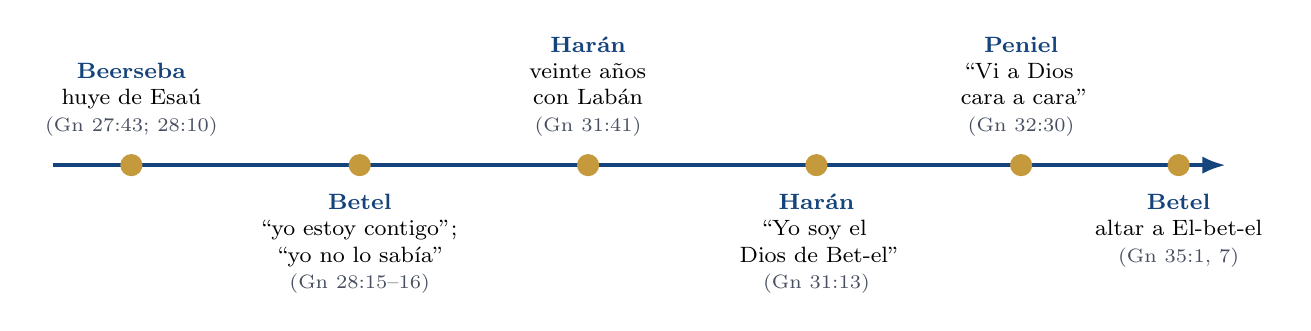
\begin{tikzpicture}[font=\footnotesize]
 \draw[line width=1.6pt,azul,-{Latex[length=3mm]}] (-0.3,0) -- (14.6,0);
 \foreach \x/\t/\b/\r/\pos in {0.7/{Beerseba}/{huye de Esaú}/{Gn 27:43; 28:10}/above,
   3.6/{Betel}/{``yo estoy contigo''; ``yo no lo sabía''}/{Gn 28:15--16}/below,
   6.5/{Harán}/{veinte años con Labán}/{Gn 31:41}/above,
   9.4/{Harán}/{``Yo soy el Dios de Bet-el''}/{Gn 31:13}/below,
   12.0/{Peniel}/{``Vi a Dios cara a cara''}/{Gn 32:30}/above,
   14.0/{Betel}/{altar a El-bet-el}/{Gn 35:1, 7}/below}{
  \fill[dorado] (\x,0) circle (4pt);
  \node[\pos=7pt,text width=2.4cm,align=center] at (\x,0) {\textbf{\textcolor{azul}{\t}}\\ \b\\ {\scriptsize\color{gris}(\r)}};}
\end{tikzpicture}\par
{\footnotesize\color{gris}\textit{Figura 7.} El Dios de Betel acompaña a Jacob. \textit{Nota.} Elaboración propia.}
\end{center}

A su regreso, Dios lo envía de nuevo a Betel: ``haz allí un altar al Dios que te apareció cuando huías de tu hermano Esaú'' (35:1). Jacob llama entonces al lugar El-bet-el, ``el Dios de Betel'' (35:7). Lo decisivo ya no es el lugar, sino el Dios del lugar.

\begin{nota}[Precisión]
La tradición rabínica lee \heb{וַיִּפְגַּע} como oración: ``y no hay \emph{pegiá} sino oración'' (\heb{וְאֵין פְּגִיעָה אֶלָּא תְּפִלָּה}), porque el mismo verbo aparece en Jer 7:16 (``ni me ruegues'', \heb{וְאַל־תִּפְגַּע־בִּי}); de ahí se concluye que Jacob instituyó la oración de la tarde (\emph{Berajot} 26b). Se trata de una interpretación rabínica, no del sentido llano del texto.
\end{nota}

%===================================================================
\section{La omnipresencia en el judaísmo}\label{sec:judaismo-omni}

\subsection{\emph{HaMaqom}: ``el Lugar del mundo''}

La literatura rabínica da a Dios un nombre ausente de la Biblia: \heb{הַמָּקוֹם} \emph{HaMaqom}, ``el Lugar''. El Midrash lo explica justamente a partir de Betel:

\hebverso{מִפְּנֵי מָה מְכַנִּין שְׁמוֹ שֶׁל הַקָּדוֹשׁ בָּרוּךְ הוּא וְקוֹרְאִין אוֹתוֹ מָקוֹם\\ שֶׁהוּא מְקוֹמוֹ שֶׁל עוֹלָם וְאֵין עוֹלָמוֹ מְקוֹמוֹ}
\begin{quote}\itshape
``Y llegó al lugar'' (Gn 28:11). Rav Huná dijo en nombre de Rabí Amí: ¿Por qué se da al Santo, bendito sea, el sobrenombre de \emph{Maqom}, ``Lugar''? Porque él es el lugar del mundo, y el mundo no es su lugar. Así está escrito: ``He aquí un lugar junto a mí'' (Éx 33:21). [\ldots] Rabí Abbá bar Yudán dijo: es como un guerrero montado a caballo, con sus armas colgando de un lado y del otro: el caballo depende del jinete, y no el jinete del caballo, como está dicho: ``cuando montaste en tus caballos'' (Hab 3:8).\par\hfill{\upshape\small\bfseries\textcolor{azul}{(\emph{Bereshit Rabá} 68:9)}}
\end{quote}

El mismo pasaje cita Dt 33:27, ``El eterno Dios es tu refugio'' (\heb{מְעֹנָה}, ``morada''), y Sal 90:1, ``Señor, tú nos has sido refugio'' (\heb{מָעוֹן}), y llega a la misma conclusión: Dios es la morada del mundo, y el mundo no es su morada.

\begin{nota}[Precisión]
Interpretación rabínica (Sefaria); traducción propia. Expresa, desde el otro extremo, la idea de 1 R 8:27: no es el mundo el que contiene a Dios, sino Dios el que contiene al mundo.
\end{nota}

El nombre pasó a la oración y a la vida cotidiana. La Misná aconseja: ``cuando ores, no hagas de tu oración algo fijo, sino misericordia y súplica delante de \emph{HaMaqom}'' (\emph{Pirké Avot} 2:13):
\hebverso{רַחֲמִים וְתַחֲנוּנִים לִפְנֵי הַמָּקוֹם}
Todavía hoy, al consolar a quien está de duelo, se le dice: ``que \emph{HaMaqom} os consuele entre los demás que lloran por Sion y Jerusalén'':
\hebverso{הַמָּקוֹם יְנַחֵם אֶתְכֶם בְּתוֹךְ שְׁאָר אֲבֵלֵי צִיּוֹן וִירוּשָׁלָיִם}
\noindent Justo cuando alguien siente a Dios más lejos, se lo nombra como ``el Lugar'': el que también está allí.

\begin{nota}[Precisión]
La fórmula de consolación es una costumbre litúrgica de la tradición asquenazí, y su redacción varía de una comunidad a otra.
\end{nota}

\subsection{``No hay lugar vacío de la Shejiná''}

La palabra \heb{שְׁכִינָה} \emph{Shejiná}, ``morada, presencia que habita'', de la raíz \heb{שׁכן}, es el término rabínico para la presencia de Dios. Tres textos permiten ver cómo la entendió el judaísmo antiguo:

\begin{center}\small\renewcommand{\arraystretch}{1.22}
\begin{tabular}{@{}L{3.0cm}L{11.0cm}@{}}
\toprule
\textbf{Fuente} & \textbf{Enseñanza} \\ \midrule
\emph{Shemot Rabá} 2:5 & Un gentil pregunta a Rabí Yehoshúa ben Korjá por qué Dios habló a Moisés desde una zarza. Respuesta: \heb{לְלַמֶּדְךָ שֶׁאֵין מָקוֹם פָּנוּי בְּלֹא שְׁכִינָה אֲפִלּוּ סְנֶה}, ``para enseñarte que no hay lugar vacío de la Shejiná, ni siquiera una zarza''. \\
\emph{Bava Batra} 25a & Rabí Oshayá: \heb{שְׁכִינָה בְּכׇל מָקוֹם}, ``la Shejiná está en todo lugar''; lo prueba con Neh 9:6: ``Tú solo eres \SENOR{}; tú hiciste los cielos\ldots{} y tú vivificas todas estas cosas''. La escuela de Rabí Ismael enseña lo mismo. \\
\emph{Sanedrín} 39a & El emperador pregunta a Rabán Gamliel: ``Decís que dondequiera que hay diez reunidos reposa la Shejiná. ¿Cuántas Shejinás hay?''. Gamliel responde con el sol: si el sol, uno de los innumerables siervos de Dios, alumbra todo el mundo, ``¡cuánto más la Shejiná del Santo, bendito sea!''. \\
\emph{Berajot} 10a & ``Como el Santo, bendito sea, llena todo el mundo, así el alma llena todo el cuerpo'' (véase el capítulo ``Dios es Espíritu''). \\
\bottomrule
\end{tabular}\par
{\footnotesize\color{gris}\textit{Tabla 9.} La Shejiná en todo lugar. \textit{Nota.} Textos según Sefaria; traducción propia.}
\end{center}

El pasaje de \emph{Sanedrín} 39a toca un punto delicado: la presencia de Dios ``en medio de diez'' no lo divide en muchas presencias. Jesús dirá algo semejante: ``donde están dos o tres congregados en mi nombre, allí estoy yo en medio de ellos'' (Mt 18:20).

\subsection{La \emph{Qedushá}: ``¿Dónde está el lugar de su gloria?''}

La oración de la sinagoga une los dos textos de la visión: el de Isaías, ``toda la tierra está llena de su gloria'' (Is 6:3), y el de Ezequiel, ``Bendita sea la gloria de \SENOR{} desde su lugar'' (\heb{בָּרוּךְ כְּבוֹד־יְהוָה מִמְּקוֹמוֹ}, Ez 3:12). Entre ambos, la \emph{Qedushá} del servicio adicional (\emph{Musaf}) intercala una frase que conserva la paradoja:

\hebverso{כְּבוֹדוֹ מָלֵא עוֹלָם מְשָׁרְתָיו שׁוֹאֲלִים זֶה לָזֶה אַיֵּה מְקוֹם כְּבוֹדוֹ}
\begin{quote}\itshape
Su gloria llena el mundo; sus servidores se preguntan unos a otros: ¿Dónde está el lugar de su gloria?\par\hfill{\upshape\small\bfseries\textcolor{azul}{(\emph{Sidur}, \emph{Qedushá} de \emph{Musaf})}}
\end{quote}

Los ángeles saben que la gloria lo llena todo y, justamente por eso, no pueden señalar un lugar. Es la misma tensión de Jer 23:23--24: el Dios cercano es también el Dios lejano.

\subsection{Los targumes: la gloria y la Shejiná}

\begin{center}\small\renewcommand{\arraystretch}{1.22}
\begin{tabular}{@{}L{3.4cm}L{10.6cm}@{}}
\toprule
\textbf{Ónkelos} (Gn 28:16) & \heb{בְּקוּשְׁטָא אִית יְקָרָא דַיְיָ שָׁרֵי בְּאַתְרָא הָדֵין}: ``En verdad la \destacar{gloria} del \SENOR{} habita en este lugar''. \\
\textbf{Jonatán} (Jer 23:24) & \heb{הֲלָא יַת שְׁמַיָא וְיַת אַרְעָא יְקָרִי מְלֵי}: ``¿No llena \destacar{mi gloria} los cielos y la tierra?''. \\
\textbf{Jonatán} (Ez 48:35) & \heb{מִיוֹמָא דִי יִשְׁרֵי יְיָ שְׁכִנְתֵּיהּ תַּמָן}: ``desde el día en que el \SENOR{} haga reposar su \destacar{Shejiná} allí''. \\
\bottomrule
\end{tabular}\par
{\footnotesize\color{gris}\textit{Tabla 10.} La presencia en los targumes. \textit{Nota.} Textos según Sefaria; traducción propia.}
\end{center}

Los targumes no niegan que Dios esté presente; lo que evitan es decir que su ser ocupe un sitio. Por eso hablan de su ``gloria'' (\heb{יְקָרָא}) o de su ``Shejiná''. Es la misma reverencia que se observó en el capítulo sobre el Espíritu, donde los targumes escriben ``la gloria'' o ``la voz'' para no decir que alguien vio a Dios.

\subsection{Maimónides: lugar y cercanía}

Maimónides dedica dos capítulos de la \emph{Guía de los perplejos} a este vocabulario. En I:8 explica que \emph{maqom} significó primero ``lugar'' y luego se extendió a ``rango, grado'', y por eso lee ``Bendita sea la gloria de \SENOR{} desde su lugar'' (Ez 3:12) como ``según la excelsitud de su existencia''. En I:18 sostiene que ``acercarse'' y ``estar cerca'', dichos de Dios, no indican proximidad física, sino conocimiento y comprensión: está cerca de Dios quien lo conoce. Se trata de una lectura filosófica, que busca proteger la incorporeidad de Dios.

\begin{nota}[Precisión]
Lectura judía medieval (Maimónides, 1903, I:8, I:18; Sefaria). La Biblia no reduce la cercanía de Dios al conocimiento, pero tampoco la concibe como distancia física: Dios está ``cerca de todos los que le invocan'' (Sal 145:18).
\end{nota}

\subsection{Qumrán: el Salmo 139 en el rollo de los Salmos}

El gran rollo de los Salmos de la cueva 11 (11QPs\textsuperscript{a}) conserva el Salmo 139 desde el versículo 8 (Sanders, 1965). La comunidad de Qumrán copiaba y oraba, pues, el salmo de la presencia ineludible. Según las transcripciones publicadas, en el versículo 10 el rollo carece de la palabra inicial \heb{גַּם} (``aun'') y dice: ``allí me guiará tu mano''.

\begin{nota}[Precisión textual]
La variante del versículo 10 se toma de las transcripciones publicadas de 11Q5; conviene cotejarla en Sanders (1965) o en la Leon Levy Dead Sea Scrolls Digital Library. En cualquier caso, no altera el sentido del versículo.
\end{nota}

%===================================================================
\section{La omnipresencia en Cristo, leída con Pablo}\label{sec:cristo-omni}

\subsection{Emanuel, de principio a fin}

El Evangelio de Mateo se abre y se cierra con la presencia. Al comienzo está el nombre: ``Emanuel, que traducido es: Dios con nosotros'' (Mt 1:23). Al final, la promesa del Resucitado:

\begin{cita}enseñándoles que guarden todas las cosas que os he mandado; y he aquí yo estoy con vosotros todos los días, hasta el fin del mundo. Amén.\fuente{(Mt 28:20)}\end{cita}

En \grc{μεθ’ ἡμῶν ὁ θεός} (1:23) y en \grc{ἐγὼ μεθ’ ὑμῶν εἰμι} (28:20) resuena el mismo ``con''. Lo que el nombre anunciaba, Jesús lo promete ahora en primera persona: su presencia acompañará a la iglesia en todas las naciones y todos los días. Una promesa así solo puede hacerla quien es Dios.

\begin{nota}[Precisión]
Que Mt 1:23 y 28:20 enmarcan el evangelio es una observación literaria compartida por muchos intérpretes, apoyada en la repetición de \grc{μετά} con el pronombre.
\end{nota}

Juan dice lo mismo con el vocabulario del tabernáculo: ``Y aquel Verbo fue hecho carne, y habitó entre nosotros'' (Jn 1:14), \grc{ἐσκήνωσεν ἐν ἡμῖν}, ``puso su tienda entre nosotros''. Y regresa a Betel cuando Jesús promete a Natanael que verá ``a los ángeles de Dios que suben y descienden sobre el Hijo del Hombre'' (Jn 1:51). La escalera de Jacob es ahora una persona: el lugar donde el cielo toca la tierra ya no es Betel, sino Jesús.

\begin{center}\small\renewcommand{\arraystretch}{1.2}
\begin{tabular}{@{}L{2.4cm}L{5.8cm}L{5.8cm}@{}}
\toprule
 & \textbf{Gn 28:12 (LXX)} & \textbf{Jn 1:51} \\ \midrule
Ángeles & \grc{οἱ ἄγγελοι τοῦ θεοῦ ἀνέβαινον καὶ κατέβαινον} & \grc{τοὺς ἀγγέλους τοῦ θεοῦ ἀναβαίνοντας καὶ καταβαίνοντας} \\
Sobre & \grc{ἐπ’ αὐτῆς}, ``sobre ella'' (la escalera) & \grc{ἐπὶ τὸν υἱὸν τοῦ ἀνθρώπου}, ``sobre el Hijo del Hombre'' \\
Lugar & ``casa de Dios, y puerta del cielo'' (28:17) & ``veréis el cielo abierto'' \\
\bottomrule
\end{tabular}\par
{\footnotesize\color{gris}\textit{Tabla 11.} Betel en Juan 1:51. \textit{Nota.} Elaboración propia a partir de Rahlfs-Hanhart (2006) y NA28.}
\end{center}

\subsection{Pablo en Atenas: ``no está lejos de cada uno de nosotros''}

Ante un auditorio griego, Pablo predica con las dos caras de Jer 23:23--24. Comienza por la inmensidad, pues Dios no cabe en templos, y pasa luego a la cercanía, pues no está lejos.

\begin{cita}El Dios que hizo el mundo y todas las cosas que en él hay, siendo Señor del cielo y de la tierra, no habita en templos hechos por manos humanas\ldots{} para que busquen a Dios, si en alguna manera, palpando, puedan hallarle, aunque ciertamente no está lejos de cada uno de nosotros. Porque en él vivimos, y nos movemos, y somos; como algunos de vuestros propios poetas también han dicho: Porque linaje suyo somos.\fuente{(Hch 17:24, 27--28)}\end{cita}

\begin{filologia}[Hch 17:27--28]
\begin{tabular}{@{}L{3.6cm}L{1.6cm}L{9.6cm}@{}}
\grc{οὐ μακρὰν} & \grc{μακρός} & ``no lejos'': la misma oposición cerca/lejos de Jer 23:23. \\[2pt]
\grc{ἀπὸ ἑνὸς ἑκάστου ἡμῶν} & --- & ``de cada uno de nosotros'': la cercanía es personal, no solo general. Pablo se incluye con los atenienses. \\[2pt]
\grc{ἐν αὐτῷ γὰρ ζῶμεν καὶ κινούμεθα καὶ ἐσμέν} & --- & ``en él vivimos, nos movemos y somos'': tres verbos que cubren la vida, la actividad y la existencia. \\[2pt]
\grc{τοῦ γὰρ καὶ γένος ἐσμέν} & --- & ``porque también somos linaje suyo'': cita del poeta Arato (\emph{Fenómenos} 5). \\
\end{tabular}
\end{filologia}

\begin{nota}[Precisión]
La frase ``Porque linaje suyo somos'' procede de Arato (\emph{Fenómenos} 5). ``En él vivimos, y nos movemos, y somos'' se atribuye a Epiménides de Creta (MacArthur, 2011, nota a Hch 17:28), atribución que descansa en fuentes posteriores y es discutida (Bruce, 1990). El discurso lo transmite Lucas, y aquí se usa como testimonio de la predicación de Pablo.
\end{nota}

Washer subraya esa misma frase: ``Sea que el hombre lo reconozca o no, la realidad de Dios es ineludible. No hay lugar en el que Él no esté'' (Washer, 2021, p. 90). Pablo, sin embargo, no invoca la omnipresencia para afirmar que todos están ya en comunión con Dios, sino para llamar al arrepentimiento: el Dios que no está lejos ``manda a todos los hombres en todo lugar, que se arrepientan'' (Hch 17:30).

\subsection{``Que todo lo llena en todo''}

En Efesios, el verbo de Jer 23:24 pasa a tener a Cristo por sujeto:

\begin{cita}y sometió todas las cosas bajo sus pies, y lo dio por cabeza sobre todas las cosas a la iglesia, la cual es su cuerpo, la plenitud de Aquel que todo lo llena en todo.\fuente{(Ef 1:22--23)}\end{cita}
\begin{cita}Y eso de que subió, ¿qué es, sino que también había descendido primero a las partes más bajas de la tierra? El que descendió, es el mismo que también subió por encima de todos los cielos para llenarlo todo.\fuente{(Ef 4:9--10)}\end{cita}

\begin{center}\small\renewcommand{\arraystretch}{1.22}
\begin{tabular}{@{}L{2.2cm}L{6.4cm}L{5.4cm}@{}}
\toprule
\textbf{Texto} & \textbf{Griego} & \textbf{Sujeto} \\ \midrule
Jer 23:24 LXX & \grc{μὴ οὐχὶ τὸν οὐρανὸν καὶ τὴν γῆν ἐγὼ πληρῶ;} & el \SENOR{} \\
Ef 1:23 & \grc{τὸ πλήρωμα τοῦ τὰ πάντα ἐν πᾶσιν πληρουμένου} & Cristo, cabeza de la iglesia \\
Ef 4:10 & \grc{ὑπεράνω πάντων τῶν οὐρανῶν, ἵνα πληρώσῃ τὰ πάντα} & Cristo, que descendió y subió \\
Ef 4:6 & \grc{ὁ ἐπὶ πάντων καὶ διὰ πάντων καὶ ἐν πᾶσιν} & ``un Dios y Padre de todos'' \\
\bottomrule
\end{tabular}\par
{\footnotesize\color{gris}\textit{Tabla 12.} El verbo ``llenar'' de Jeremías a Efesios. \textit{Nota.} Elaboración propia a partir de Rahlfs-Hanhart (2006) y NA28.}
\end{center}

Lo que en Jeremías es prerrogativa del \SENOR{}, ``yo lleno el cielo y la tierra'', en Efesios es obra de Cristo exaltado, que subió ``por encima de todos los cielos para llenarlo todo''. Al descender ``a las partes más bajas'' y subir sobre todos los cielos, Cristo recorre los extremos del Salmo 139: lo alto y lo profundo. MacArthur comenta que, tras su ascensión, Cristo ``había llegado a llenar el universo entero con su presencia, su poder, su soberanía y su bendición como Dios mismo'' (MacArthur, 2011, nota a Ef 4:10).

\begin{nota}[Precisión]
La autoría paulina de Efesios se discute. En Ef 1:23 el participio \grc{πληρουμένου} admite una lectura en voz media (``que llena'') o pasiva (``que es llenado''); la RVR1960 sigue la media, y Lincoln (1990) resume la discusión. La idea de Cristo como mediador de toda la creación aparece también en una carta indiscutida: ``un Señor, Jesucristo, por medio del cual son todas las cosas'' (1 Co 8:6).
\end{nota}

\subsection{``Cerca de ti está la palabra''}

En Romanos, Pablo retoma un texto de Moisés que suena al Salmo 139 y lo lee a la luz de Cristo:

\begin{center}\small\renewcommand{\arraystretch}{1.22}
\begin{tabular}{@{}L{4.6cm}L{4.6cm}L{4.8cm}@{}}
\toprule
\textbf{Dt 30:12--14} & \textbf{Ro 10:6--8} & \textbf{Lectura de Pablo} \\ \midrule
``¿Quién subirá por nosotros al cielo?'' & ``¿Quién subirá al cielo?'' & ``esto es, para traer abajo a Cristo'' \\
``¿Quién pasará por nosotros el mar?'' & ``¿quién descenderá al abismo?'' & ``esto es, para hacer subir a Cristo de entre los muertos'' \\
``muy cerca de ti está la palabra, en tu boca y en tu corazón'' & ``Cerca de ti está la palabra, en tu boca y en tu corazón'' & ``Esta es la palabra de fe que predicamos'' \\
\bottomrule
\end{tabular}\par
{\footnotesize\color{gris}\textit{Tabla 13.} Dt 30 en Romanos 10. \textit{Nota.} Elaboración propia; textos de la RVR1960.}
\end{center}

Para encontrar a Dios no hace falta subir al cielo ni bajar al abismo, porque Cristo ya bajó y ya subió. Lo que Dt 30 afirmaba del mandamiento, Pablo lo afirma de Cristo anunciado: \grc{ἐγγύς σου τὸ ῥῆμά ἐστιν}, ``cerca de ti está la palabra''. Hays (1989) estudia este pasaje como muestra de la manera en que Pablo relee la Escritura de Israel a la luz de Cristo.

\begin{nota}[Precisión]
Pablo sustituye ``el mar'' de Dt 30:13 por ``el abismo'' (\grc{ἄβυσσος}), quizá por influencia de textos como Sal 107:26 o de la tradición judía que leía Dt 30 en clave de altura y profundidad. El eco del Salmo 139:8 (cielos y Seol) es una lectura posible, no explícita.
\end{nota}

\subsection{Ni lo alto ni lo profundo}

Romanos 8 se cierra con una enumeración que recorre el universo, como la del Salmo 139:

\begin{cita}Por lo cual estoy seguro de que ni la muerte, ni la vida, ni ángeles, ni principados, ni potestades, ni lo presente, ni lo por venir, ni lo alto, ni lo profundo, ni ninguna otra cosa creada nos podrá separar del amor de Dios, que es en Cristo Jesús Señor nuestro.\fuente{(Ro 8:38--39)}\end{cita}

``Ni lo alto, ni lo profundo'' (\grc{οὔτε ὕψωμα οὔτε βάθος}). El salmista no hallaba lugar donde huir de Dios; Pablo no halla lugar adonde no alcance el amor de Dios en Cristo. Vista desde la cruz, la omnipresencia se convierte en seguridad.

\begin{nota}[Precisión]
\grc{ὕψωμα} y \grc{βάθος} pueden ser términos astrológicos (las regiones del cielo por encima y por debajo del horizonte), como señala Moo (1996); en cualquier caso, abarcan todo el espacio creado. La relación con el Salmo 139 es un posible eco.
\end{nota}

\subsection{El templo que es un pueblo}

La presencia que Israel conoció en el tabernáculo y en el templo, Pablo la reconoce ahora en la iglesia:

\begin{cita}¿No sabéis que sois templo de Dios, y que el Espíritu de Dios mora en vosotros?\fuente{(1 Co 3:16)}\end{cita}
\begin{cita}¿Y qué acuerdo hay entre el templo de Dios y los ídolos? Porque vosotros sois el templo del Dios viviente, como Dios dijo: Habitaré y andaré entre ellos, Y seré su Dios, Y ellos serán mi pueblo.\fuente{(2 Co 6:16)}\end{cita}

Pablo cita aquí Lv 26:11--12 (``andaré entre vosotros'') y Ez 37:27 (``Estará en medio de ellos mi tabernáculo''): \grc{ἐνοικήσω ἐν αὐτοῖς καὶ ἐμπεριπατήσω}. El Dios que llena el cielo y la tierra se compromete a habitar en un pueblo formado por judíos y gentiles, edificado ``para morada de Dios en el Espíritu'' (Ef 2:22). Así se cumple \SENOR{}-sama: Dios está allí, en medio de los suyos.

\subsection{``El Señor está cerca''}

\begin{cita}Vuestra gentileza sea conocida de todos los hombres. El Señor está cerca.\fuente{(Flp 4:5)}\end{cita}

La expresión \grc{ὁ κύριος ἐγγύς} reproduce el \grc{ἐγγὺς κύριος} del Sal 144:18 LXX (145:18 en hebreo y en español), ``Cercano está el \SENOR{} a todos los que le invocan''. El versículo siguiente lo confirma: ``Por nada estéis afanosos, sino sean conocidas vuestras peticiones delante de Dios en toda oración'' (Flp 4:6). La cercanía del Señor es, por tanto, la razón para orar en lugar de angustiarse.

\begin{nota}[Precisión]
``Cerca'' puede tener sentido temporal (la venida del Señor está próxima; cf. Ro 13:12) o espacial (el Señor está presente). Fee (1995) ve aquí un eco del Sal 145:18 sin excluir el sentido temporal. Ambas lecturas son compatibles.
\end{nota}

\subsection{Cristo y la omnipresencia: una precisión teológica}

Si Cristo es verdadero hombre y tiene un cuerpo resucitado, ¿cómo puede estar ``con vosotros todos los días''? La tradición reformada responde que el Hijo llena el mundo según su naturaleza divina, mientras que su humanidad glorificada está en un lugar; la tradición luterana, en cambio, afirma que la humanidad de Cristo participa de la omnipresencia de su divinidad.

\begin{nota}[Precisión]
Calvino lo expresa así: ``el Hijo de Dios descendió del cielo de tal modo que, sin dejar el cielo, quiso nacer en el vientre de la virgen, andar por la tierra y ser colgado en la cruz; y sin embargo llenaba continuamente el mundo, como lo había hecho desde el principio'' (Calvino, 1960, II, 13, 4; traducción propia). La posición luterana se formula en la \emph{Fórmula de Concordia} (1577), artículo VIII (Kolb y Wengert, 2000). Se trata de un debate entre tradiciones cristianas, que la serie no pretende resolver aquí.
\end{nota}

\subsection{Síntesis paulina}

\begin{center}
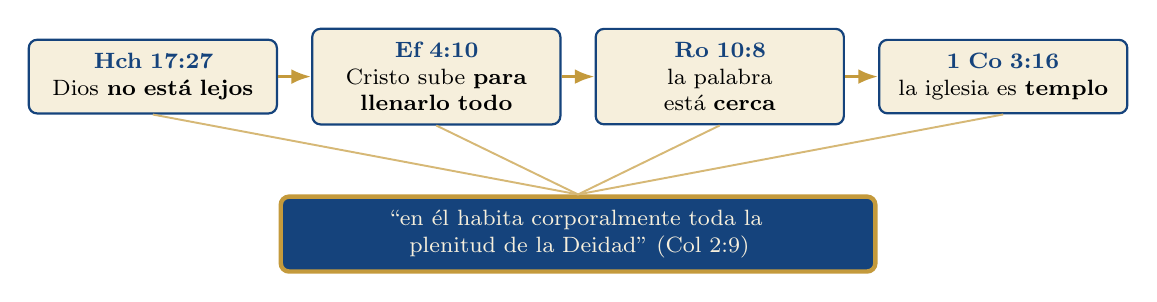
\begin{tikzpicture}[font=\footnotesize]
 \foreach \x/\n/\t/\d in {0/a/{Hch 17:27}/{Dios \textbf{no está lejos}},
   3.6/b/{Ef 4:10}/{Cristo sube \textbf{para llenarlo todo}},
   7.2/c/{Ro 10:8}/{la palabra está \textbf{cerca}},
   10.8/d/{1 Co 3:16}/{la iglesia es \textbf{templo}}}{
  \node[draw=azul,line width=0.8pt,fill=papiro,rounded corners=3pt,text width=2.8cm,align=center,inner sep=5pt] (\n) at (\x,0) {\textbf{\textcolor{azul}{\t}}\\ \d};}
 \draw[-{Latex[length=2.5mm]},dorado,line width=1.1pt](a)--(b); \draw[-{Latex[length=2.5mm]},dorado,line width=1.1pt](b)--(c); \draw[-{Latex[length=2.5mm]},dorado,line width=1.1pt](c)--(d);
 \node[draw=dorado,line width=1.6pt,fill=azul,text=papiro,rounded corners=3pt,text width=7.2cm,align=center,inner sep=5pt] (e) at (5.4,-2.0) {``en él habita corporalmente toda la plenitud de la Deidad'' (Col 2:9)};
 \foreach \i in {a,b,c,d}\draw[dorado!70,line width=0.7pt](\i.south)--(e.north);
\end{tikzpicture}\par
{\footnotesize\color{gris}\textit{Figura 8.} La omnipresencia de Dios revelada en Cristo, según Pablo. \textit{Nota.} Elaboración propia.}
\end{center}

Pablo, judío formado en Jeremías y en los Salmos, nunca deja de confesar que Dios llena el cielo y la tierra. Pero ahora sabe dónde ese Dios se deja encontrar: en Cristo, que descendió y subió; en la palabra predicada, que está cerca; y en el pueblo donde habita por su Espíritu. \SENOR{}-sama tiene ya nombre propio: Emanuel.

%===================================================================
\section{Aplicación: vivir delante de Dios}

\subsection{No hay dónde huir}

Jonás intentó lo que el Salmo 139 declara imposible. ``Se levantó para huir de la presencia de \SENOR{} a Tarsis'' (Jon 1:3), el extremo occidental del mundo conocido. Bajó a Jope, bajó a la nave, bajó al fondo del barco (\heb{וַיֵּרֶד}, \heb{יָרַד}; Jon 1:3, 5) y acabó en el mar. Y desde el lugar más bajo, ``desde el vientre del pez'', oró: ``Desde el seno del Seol clamé, y mi voz oíste'' (Jon 2:1--2 [2:2--3]). El que huía de la presencia descubrió que la presencia lo aguardaba en el Seol. Ya Adán y Eva ``se escondieron de la presencia de \SENOR{} Dios entre los árboles del huerto'' (Gn 3:8), y Dios salió a buscarlos. Huir de Dios es imposible; volver a él, en cambio, siempre es posible.

\subsection{No hay pecado oculto}

``Los ojos de \SENOR{} están en todo lugar, mirando a los malos y a los buenos'' (Pr 15:3). José, solo en la casa de Potifar y sin testigos, respondió: ``¿cómo, pues, haría yo este grande mal, y pecaría contra Dios?'' (Gn 39:9). La santidad en lo secreto brota de saber que nada es secreto delante de Dios; Pink lo llama un ``freno'' (Pink, 2020, cap. 3, p. 19).

\subsection{No hay soledad sin Dios}

``Cuando pases por las aguas, yo estaré contigo\ldots{} Cuando pases por el fuego, no te quemarás'' (Is 43:2). ``Aunque ande en valle de sombra de muerte, no temeré mal alguno, porque tú estarás conmigo'' (Sal 23:4). La carta a los Hebreos recurre a Dt 31:6 para exhortar al contentamiento: ``porque él dijo: No te desampararé, ni te dejaré'' (He 13:5). La presencia de Dios no suprime el valle, pero transforma a quien lo atraviesa.

\subsection{No hay lugar donde no se pueda orar}

Jacob encontró a Dios mientras dormía en el campo, y Jonás oró desde el vientre del pez. Jesús mandó: ``cuando ores, entra en tu aposento, y cerrada la puerta, ora a tu Padre que está en secreto'' (Mt 6:6), y Pablo quiere ``que los hombres oren en todo lugar'' (1 Ti 2:8). La sala de un hospital, una cocina, un bus o una cárcel pueden convertirse en Betel.

\subsection{No hay rincón fuera de la misión}

La promesa ``yo estoy con vosotros todos los días'' va unida al mandato ``id, y haced discípulos a todas las naciones'' (Mt 28:19--20). La presencia de Cristo no es solo un consuelo para quedarse, sino la razón para ir. No existe pueblo, barrio ni lengua donde Cristo no esté antes que el mensajero.

\subsection{Cinco respuestas}

\begin{center}
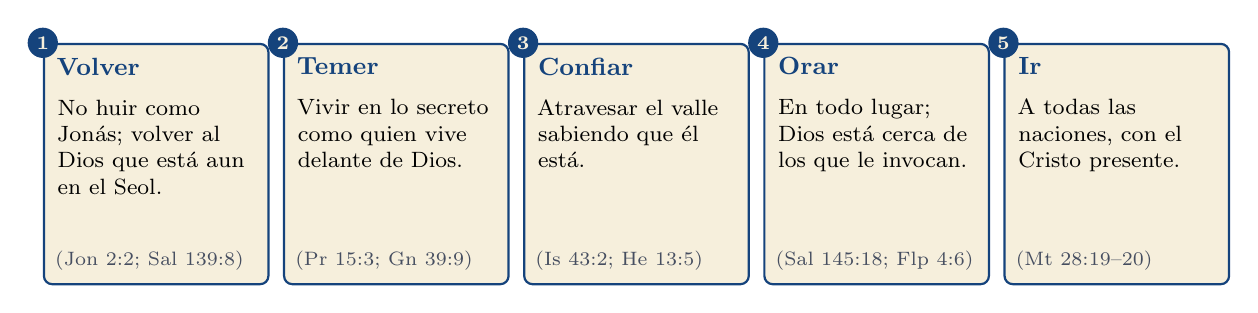
\begin{tikzpicture}
 \foreach \x/\n/\t/\d/\r in {0/1/{Volver}/{No huir como Jonás; volver al Dios que está aun en el Seol.}/{Jon 2:2; Sal 139:8},
   3.05/2/{Temer}/{Vivir en lo secreto como quien vive delante de Dios.}/{Pr 15:3; Gn 39:9},
   6.1/3/{Confiar}/{Atravesar el valle sabiendo que él está.}/{Is 43:2; He 13:5},
   9.15/4/{Orar}/{En todo lugar; Dios está cerca de los que le invocan.}/{Sal 145:18; Flp 4:6},
   12.2/5/{Ir}/{A todas las naciones, con el Cristo presente.}/{Mt 28:19--20}}{
  \node[draw=azul,line width=0.8pt,fill=papiro,rounded corners=3pt,inner sep=5pt,anchor=north] (b\n) at (\x,0) {\parbox[t][2.7cm][t]{2.5cm}{\RaggedRight
    {\small\textbf{\textcolor{azul}{\t}}}\\[5pt]\footnotesize \d\par\vfill{\scriptsize\color{gris}(\r)}}};
  \node[circle,fill=azul,text=papiro,font=\scriptsize\bfseries,inner sep=1.6pt] at (b\n.north west) {\n};}
\end{tikzpicture}\par
{\footnotesize\color{gris}\textit{Figura 9.} Cinco respuestas al Dios presente. \textit{Nota.} Elaboración propia.}
\end{center}

%===================================================================
\section{Síntesis}

\begin{tcolorbox}[colback=papiro,colframe=azul,boxrule=1pt,arc=3pt]
``¿No lleno yo, dice \SENOR{}, el cielo y la tierra?'' (Jer 23:24). Dios es aquel a quien ningún lugar contiene (1 R 8:27) y que está en todo lugar con todo su ser. Israel no tuvo una palabra para decirlo, y lo dijo con un rostro que acompaña (\emph{panim}), con un ``allí'' presente en cada extremo (\emph{sham}), con un ``contigo'' (\emph{im}) y un ``cerca'' (\emph{qarov}). En Betel, Jacob descubrió que ``el \SENOR{} está en este lugar, y yo no lo sabía'' (Gn 28:16), y el judaísmo llamó a Dios \emph{HaMaqom}, ``el Lugar del mundo''. El Nombre del atributo es \SENOR{}-sama, ``el \SENOR{} está allí'' (Ez 48:35), y su cumplimiento es Emanuel. Pablo lo reconoce en Cristo, que descendió y subió ``para llenarlo todo'' (Ef 4:10), en la palabra que está cerca (Ro 10:8) y en la iglesia, templo del Dios viviente (2 Co 6:16).
\end{tcolorbox}

\begin{center}\small\renewcommand{\arraystretch}{1.3}
\begin{tabular}{@{}L{3.0cm}L{11.4cm}@{}}
\toprule
\textbf{Mirada} & \textbf{Aporte al atributo} \\ \midrule
Hebrea & Las tres preguntas de Jer 23:23--24; \emph{panim}, \emph{sham}, \emph{im}, \emph{qarov}, \emph{maqom}, \emph{male'}, \emph{kul}; ``allí estás tú'' (Sal 139:8); ``no te pueden contener'' (1 R 8:27); \SENOR{}-sama (Ez 48:35); Betel (Gn 28). \\
Judía & \emph{HaMaqom}, el lugar del mundo (\emph{Bereshit Rabá} 68:9); ninguna zarza sin Shejiná (\emph{Shemot Rabá} 2:5); ``la Shejiná está en todo lugar'' (\emph{Bava Batra} 25a); la \emph{Qedushá}; los targumes: ``la gloria'', ``la Shejiná''; Maimónides; el Sal 139 en Qumrán. \\
Teológica & Omnipresente porque es Espíritu (Jn 4:24); inmenso: ningún lugar lo contiene (1 R 8:27); presente como Rey, no ``en todas partes salvo en su trono'' (Is 66:1); presencia que ve (Pr 15:3); Agustín, Charnock, Berkhof, Washer. \\
Paulina & El Dios no lejano (Hch 17:27); Cristo que todo lo llena (Ef 1:23; 4:10); la palabra cercana (Ro 10:8); ni lo alto ni lo profundo (Ro 8:39); el templo (1 Co 3:16; 2 Co 6:16); ``el Señor está cerca'' (Flp 4:5). \\
\bottomrule
\end{tabular}\end{center}

\begin{cita}Mas alábese en esto el que se hubiere de alabar: en entenderme y conocerme, que yo soy \SENOR{}, que hago misericordia, juicio y justicia en la tierra; porque estas cosas quiero, dice \SENOR{}.\fuente{(Jer 9:24 [9:23])}\end{cita}

``Entenderme y conocerme'': el profeta que transmitió esta invitación es el mismo que transmitió la pregunta ``¿No lleno yo el cielo y la tierra?''. Conocer al Dios presente en todo lugar significa dejar de buscar un sitio donde esconderse y comenzar a vivir delante de él, en cualquier sitio.

%===================================================================
\section*{Compendio bíblico}
\begin{center}\small\renewcommand{\arraystretch}{1.12}
\begin{tabular}{@{}L{2.2cm}L{5.0cm}|L{2.2cm}L{5.0cm}@{}}
\toprule
Gn 28:15 & ``yo estoy contigo'' & Mt 1:23 & ``Dios con nosotros'' \\
Gn 28:16 & ``\SENOR{} está en este lugar'' & Mt 18:20 & ``allí estoy yo en medio de ellos'' \\
Éx 33:14 & ``Mi presencia irá contigo'' & Mt 28:20 & ``yo estoy con vosotros todos los días'' \\
Dt 4:7 & ``dioses tan cercanos'' & Jn 1:14 & ``habitó entre nosotros'' \\
Dt 4:39 & ``arriba en el cielo y abajo en la tierra'' & Jn 1:51 & ``ángeles\ldots{} sobre el Hijo del Hombre'' \\
1 R 8:27 & ``no te pueden contener'' & Hch 17:27--28 & ``no está lejos de cada uno'' \\
Sal 139:7--12 & ``allí estás tú'' & Ro 8:39 & ``ni lo alto, ni lo profundo'' \\
Sal 145:18 & ``Cercano está \SENOR{}'' & Ro 10:8 & ``Cerca de ti está la palabra'' \\
Pr 15:3 & ``en todo lugar'' & 1 Co 3:16 & ``sois templo de Dios'' \\
Is 6:3 & ``llena de su gloria'' & 2 Co 6:16 & ``Habitaré y andaré entre ellos'' \\
Is 7:14 & ``Emanuel'' & Ef 1:23 & ``que todo lo llena en todo'' \\
Is 57:15 & ``en la altura\ldots{} y con el quebrantado'' & Ef 4:10 & ``para llenarlo todo'' \\
Jer 23:23--24 & ``¿No lleno yo\ldots{} el cielo y la tierra?'' & Flp 4:5 & ``El Señor está cerca'' \\
Ez 48:35 & ``\SENOR{}-sama'' & Ap 21:3 & ``el tabernáculo de Dios con los hombres'' \\
Am 9:2--3 & ``de allá los tomará mi mano'' & He 13:5 & ``No te desampararé'' \\
Jon 1:3 & ``para huir de la presencia'' & Stg 4:8 & ``Acercaos a Dios'' \\
\bottomrule
\end{tabular}\par
{\footnotesize\color{gris}\textit{Tabla 14.} Compendio bíblico del atributo. \textit{Nota.} Textos de la RVR1960.}
\end{center}

%===================================================================
\section*{Glosario}
\begin{description}\setlength{\itemsep}{2pt}
\item[\emph{Coram Deo}] (latín). ``Delante de Dios'': vivir sabiendo que todo ocurre en su presencia.
\item[\emph{Engýs}] (\grc{ἐγγύς}). Cerca (Sal 144:18 LXX; Ro 10:8; Flp 4:5).
\item[\emph{HaMaqom}] (\heb{הַמָּקוֹם}). ``El Lugar'': nombre rabínico de Dios, ``el lugar del mundo'' (\emph{Bereshit Rabá} 68:9).
\item[\emph{Im}] (\heb{עִם}). Con; en la promesa ``yo estoy contigo'' (Gn 28:15) y en Emanuel (Is 7:14).
\item[Inmensidad] Perfección por la que ningún espacio contiene ni limita a Dios (1 R 8:27).
\item[\emph{Kul}] (\heb{כּוּל}). Contener, abarcar; ``no te pueden contener'' (1 R 8:27).
\item[\emph{Male'}] (\heb{מָלֵא}). Llenar, estar lleno (Is 6:3; Jer 23:24).
\item[\emph{Maqom}] (\heb{מָקוֹם}). Lugar (Gn 28:11--19; Pr 15:3).
\item[Omnipresencia] Perfección por la que Dios está presente con todo su ser en todo lugar (Jer 23:24).
\item[\emph{Panim}] (\heb{פָּנִים}). Rostro, presencia; \emph{lifné}, ``delante de'' (Éx 33:14).
\item[\emph{Páreimi}] (\grc{πάρειμι}). Estar presente (Sal 138:8 LXX).
\item[\emph{Plēróō}] (\grc{πληρόω}). Llenar (Jer 23:24 LXX; Ef 4:10).
\item[\emph{Qarov}] (\heb{קָרוֹב}). Cercano (Dt 4:7; Sal 145:18; Jer 23:23).
\item[\emph{Sham}] (\heb{שָׁם}). Allí (Sal 139:8, 10; Ez 48:35).
\item[Shejiná] (\heb{שְׁכִינָה}). Término rabínico para la presencia de Dios que habita (\emph{Bava Batra} 25a).
\item[\emph{Sullam}] (\heb{סֻלָּם}). Escalera o rampa; solo en Gn 28:12.
\end{description}

\section*{Referencias}
\refapa{Agustín de Hipona. (s.f.). \emph{Confesiones} [I, 3, 3]. (Obra original escrita ca. 397--400)}
\refapa{Berkhof, L. (1938). \emph{Systematic theology}. Eerdmans.}
\refapa{Bruce, F.~F. (1990). \emph{The Acts of the Apostles: The Greek text with introduction and commentary} (3.ª ed.). Eerdmans.}
\refapa{Calvino, J. (1960). \emph{Institutes of the Christian religion} (J.~T. McNeill, Ed.; F.~L. Battles, Trad.). Westminster Press. (Obra original publicada en 1559)}
\refapa{Elliger, K., \& Rudolph, W. (Eds.). (1997). \emph{Biblia Hebraica Stuttgartensia} (5.ª ed.). Deutsche Bibelgesellschaft.}
\refapa{Fee, G.~D. (1995). \emph{Paul's letter to the Philippians}. Eerdmans.}
\refapa{Hays, R.~B. (1989). \emph{Echoes of Scripture in the letters of Paul}. Yale University Press.}
\refapa{Henry, M. (1999). \emph{Comentario bíblico de Matthew Henry} (F. Lacueva, Trad.). Editorial CLIE.}
\refapa{Kolb, R., \& Wengert, T.~J. (Eds.). (2000). \emph{The Book of Concord: The confessions of the Evangelical Lutheran Church}. Fortress Press.}
\refapa{Lincoln, A.~T. (1990). \emph{Ephesians} (Word Biblical Commentary 42). Word Books.}
\refapa{MacArthur, J. (2011). \emph{Biblia de estudio MacArthur} (notas). Grupo Nelson.}
\refapa{Maimónides. (1903). \emph{The guide for the perplexed} (M. Friedländer, Trad.; 2.ª ed.) [I, 8; I, 18]. Sefaria. https://www.sefaria.org}
\refapa{\emph{Midrash Rabá}: \emph{Bereshit Rabá} [68:9]; \emph{Shemot Rabá} [2:5]. (s.f.). Sefaria. https://www.sefaria.org}
\refapa{\emph{Misná: Pirké Avot} [2:13]. (s.f.). Sefaria. https://www.sefaria.org}
\refapa{Moo, D.~J. (1996). \emph{The epistle to the Romans}. Eerdmans.}
\refapa{Nestle, E., \& Aland, K. (Eds.). (2012). \emph{Novum Testamentum Graece} (28.ª ed.). Deutsche Bibelgesellschaft.}
\refapa{Pink, A. W. (2020). \emph{Los atributos de Dios} (E. Rodríguez Cruz, Trad.). Chapel Library. (Obra original publicada en 1930)}
\refapa{Rahlfs, A., \& Hanhart, R. (Eds.). (2006). \emph{Septuaginta} (Ed. rev.). Deutsche Bibelgesellschaft.}
\refapa{Sanders, J.~A. (1965). \emph{The Psalms scroll of Qumrân Cave 11 (11QPs\textsuperscript{a})} (Discoveries in the Judaean Desert IV). Clarendon Press.}
\refapa{\emph{Santa Biblia: Reina-Valera 1960}. (1960). Sociedades Bíblicas en América Latina.}
\refapa{\emph{Sidur asquenazí} [\emph{Qedushá} de \emph{Musaf}]. (s.f.). Sefaria. https://www.sefaria.org}
\refapa{Steinsaltz, A. (Ed.). (2017). \emph{Koren Talmud Bavli: Edición William Davidson} [Bava Batra 25a; Berajot 10a, 26b; Sanedrín 39a]. Sefaria. https://www.sefaria.org}
\refapa{\emph{Targum Ónkelos} [Gn 28:16]; \emph{Targum Jonatán a los Profetas} [Jer 23:23--24; Ez 48:35]. (s.f.). Sefaria. https://www.sefaria.org}
\refapa{Vine, W.~E. (1999). \emph{Diccionario expositivo de palabras del Antiguo y del Nuevo Testamento exhaustivo}. Caribe.}
\refapa{Washer, P.~D. (2021). \emph{Conociendo al Dios vivo} (A. Ávila, A. Valverde y J. Namnún, Trads.). Editorial Legado Bautista Confesional; HeartCry Missionary Society. (Obra original publicada en 2016)}

\end{document}
